\chapter{Membrane potential heterogeneity at the mitochondrial tubule level}\label{ch:four}
\clearpage
\section{Introduction}
Mitochondria are double membrane organelles consisting of an outer membrane and an inner membrane. The inner mitochondrial membrane (IMM) is impermeable to most ions and metabolites. There are two distinct regions of the inner membrane \cite{vogel_dynamic_2006}, the inner boundary membrane and the cristae membrane (\Fref{fig:tubeultra}). The cristae membrane forms invaginations into the matrix and represents the majority of the surface area of the IMM. Electron transport chain (ETC) and oxidative phosphorylation (OXPHOS) proteins are concentrated in the cristae \cite{benard_ultrastructure_2008}. This enrichment in the cristae is thought to mediate efficient synthesis of ATP \cite{frey_insight_2002}.

Advances in imaging techniques in the last decade have enabled research into the changes in the IMM structure in relation to the bioenergetic and disease state of the mitochondria. Mitochondria in State 3 (high respiration, ATP synthesis activity) have increased number and size of cristae compared to mitochondria in State 4 (low respiration, no ATP synthesis). Abnormal cristae morphology is observed in mitochondrial diseases such as Leber hereditary optic neuropathy (LHON) \cite{burte_disturbed_2015} and neurodegenerative diseases such as Huntington's and Parkinson's disease \cite{yu_mutant_2003,sharma_neuroprotective_2003}. 
%
\begin{figure}[htp]
	\centering
    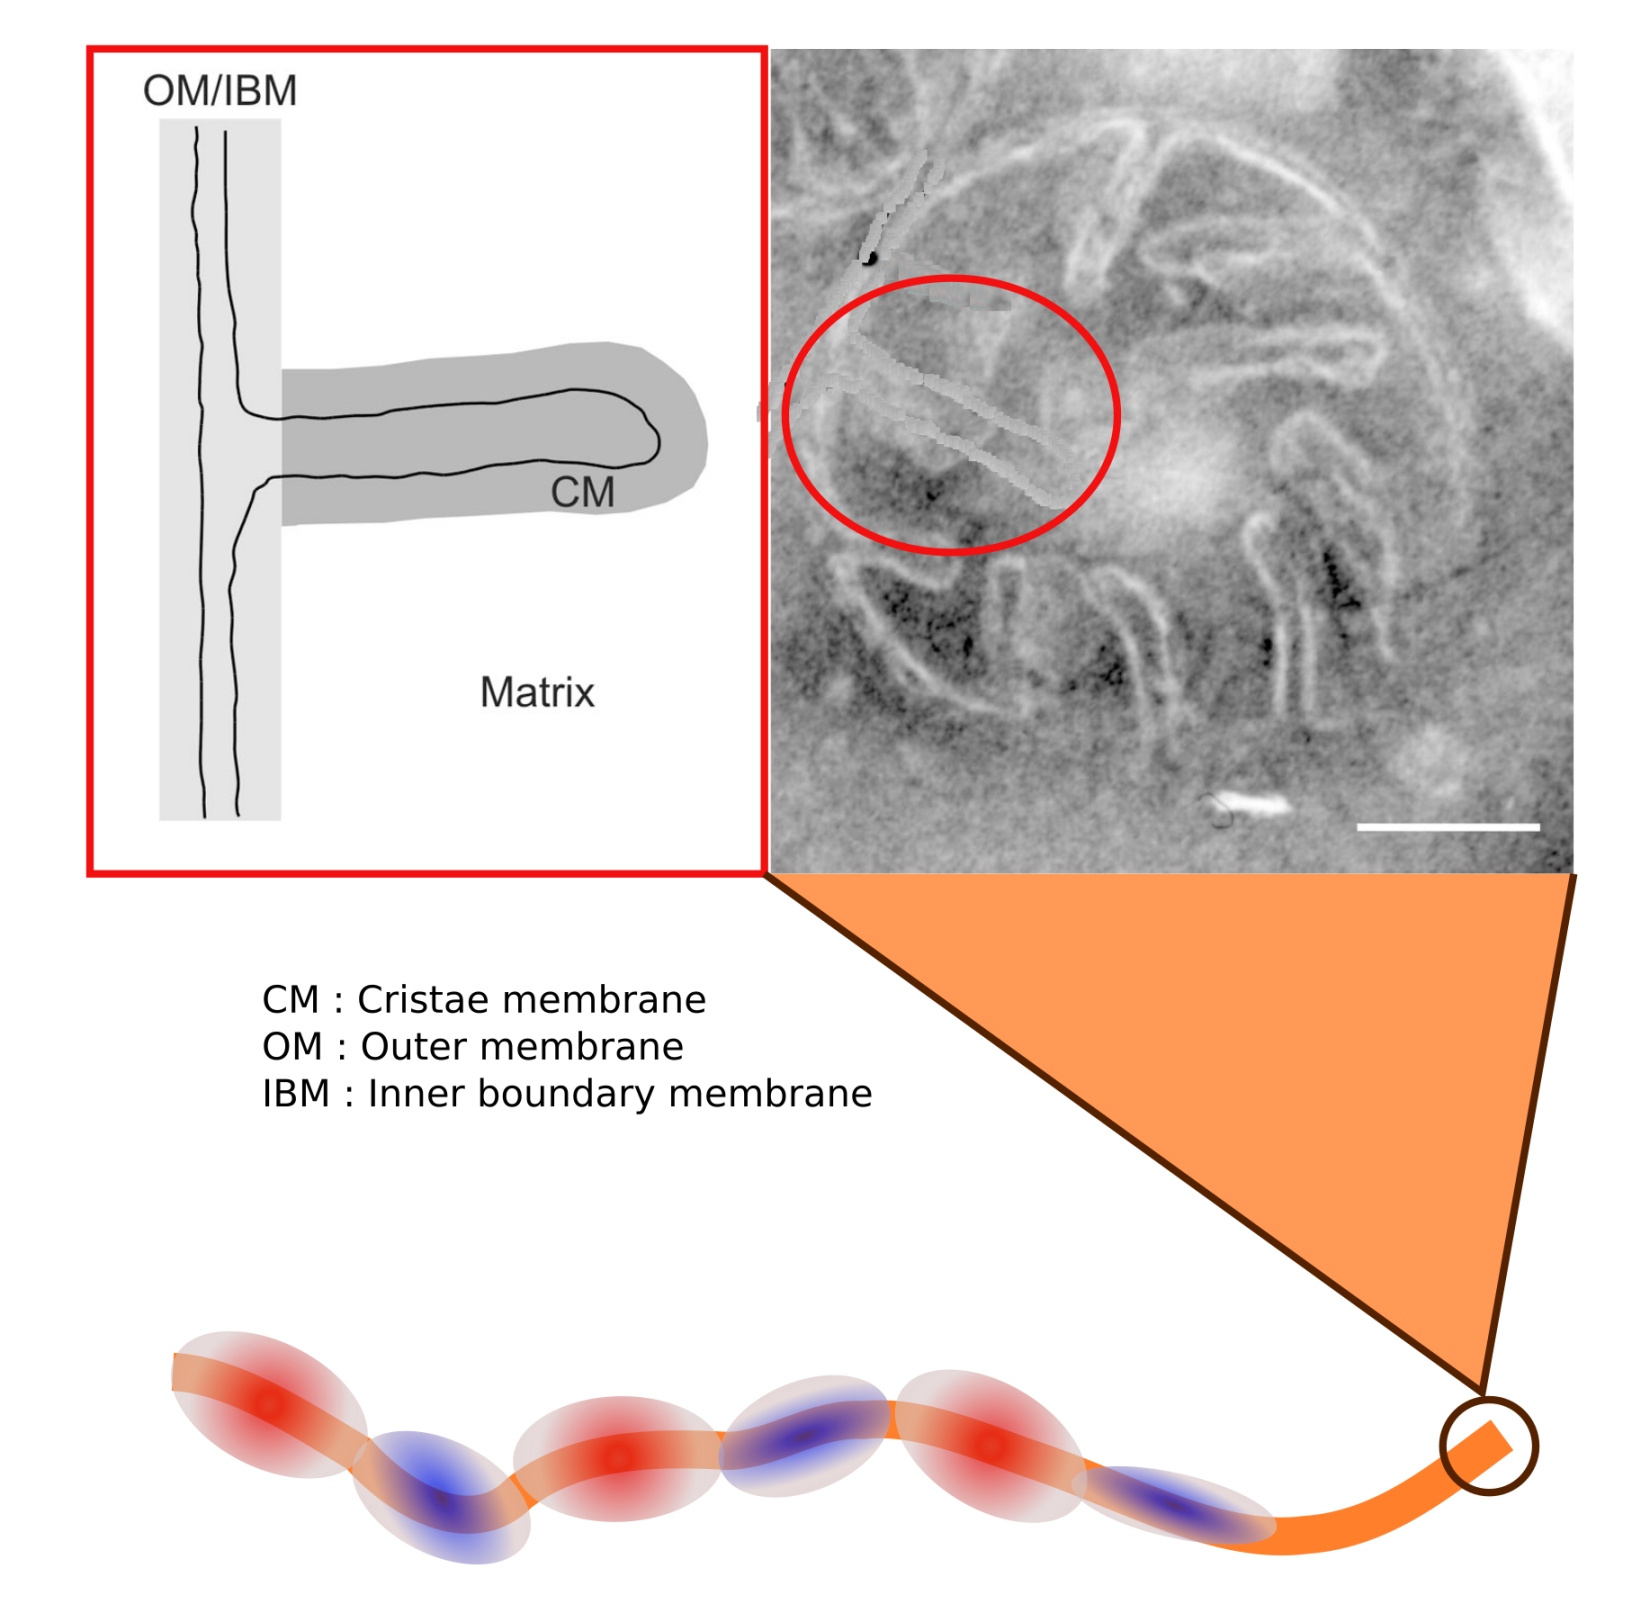
\includegraphics[width=\textwidth]{tubeultra}
    \caption[Inner mitochondrial membrane structure contributes to ΔΨ heterogeneity]{Inner mitochondrial membrane structure contributes to ΔΨ heterogeneity.\\Shown in this figure is a mitochondrial tubule displaying ΔΨ heterogeneity (higher ΔΨ levels in red, lower ΔΨ in blue). A transmission electron microscope (TEM) cross section of a real yeast mitochondrial tubule is shown in the top right image. The image was from a chemically fixed, immuno gold labeled cryosection of yeast grown in 2\% lactate. The double membrane structure of the mitochondria is visible (white edges) and the ultrastructure detail of a cristae region is shown in the top left image. Scale bar: 100 nm\\\emph{TEM images adapted from Figure 1 of Vogel et al., "Dynamic subcompartmentalization of the mitochondrial inner membrane", J Cell Biol 2006, doi:10.1083/jcb.200605138}}\label{fig:tubeultra}
\end{figure}
%

The quality and bioenergetic state of mitochondria is intimately linked to mitochondrial membrane potential (ΔΨ). The electric potential generated across the inner membrane by ΔΨ provides the energy potential to drive ATP synthesis, as well as playing a role in ROS production, mitochondrial fusion dynamics \cite{twig_mitochondrial_2008} and mitochondrial biogenesis via protein import. It has been proposed that cristae can effectively create a high resistance narrowing of the matrix lumen, effectively compartmentalizing the mitochondria into electrically distinct regions \cite{frey_insight_2002}. This would make it possible to observe heterogeneous distributions of ΔΨ within a single mitochondrial tubule due to this electrical compartmentalization by the cristae. This is thought to benefit ATP synthesis by providing a local region of high proton motive force near the cristae membrane \cite{song_biophysical_2013}, where the majority of the OXPHOS proteins are located. Whether ΔΨ can actually form heterogeneous distributions in a single mitochondrial unit is an active research field \cite{collins_mitochondria_2002,kuznetsov_heterogeneity_2009,twig_tagging_2006} because of the significance of the relationship between mitochondrial network structure and function in health and disease \cite{twig_tagging_2006}.  The following is a brief summary of previous studies on the distribution of ΔΨ within a mitochondrial tubule.

One study claimed that the ΔΨ field is equipotential across a single mitochondrial network \cite{amchenkova_coupling_1988}. They showed this by laser photobleaching a small area of the network and observed that the rest of the network promptly depolarized. Other studies found that staining with JC-1 (a ratiometric membrane potential dependent dye) resulted in significant voltage gradients along a single mitochondrial tubule \cite{bereiter1999single,smiley_intracellular_1991}. Neither studies are conclusive because firstly a diffuse depolarization of ΔΨ on local damage does not necessarily imply a homogeneous distribution of ΔΨ, while the JC-1 dye has been known to display aggregation artifacts.

One study provided evidence for the existence of discrete domains of ATP synthase cluster located at the inner membrane invaginations \cite{jimenez_mitochondrial_2014}. It is not hard to imagine that there might exist a local concentration of ΔΨ where these ATP clusters are located. One of the very first studies on ΔΨ heterogeneity within a single mitochondrial segment used human fibroblasts and astrocyte cells stained with a Nernstian membrane potential dye, TMRM \cite{diaz_homogeneous_2000}. They picked several distinct segments of mitochondria from a single cell and plotted the distributions of the ΔΨ within each mitochondrial segment. They found that the inter-mitochondrial ΔΨ variance was much higher than the variance within a single mitochondrial segment, and based on this result concluded that the ΔΨ distribution was homogeneous within a single segment. However it is not clear that all of the individual mitochondrial segments picked were really distinct units, because mitochondria in mammalian cells tend to pile up and are difficult to separate out even by eye. Indeed their own data showed that for several mitochondrial segments adjacent to each other, the variation in ΔΨ was high between these segments.

The difficulty in establishing a consistent pattern of heterogeneity is due in part to a lack of using the proper quantitative tools to establish a baseline 'control' distribution of ΔΨ within a mitochondrial tubule. Without a baseline the previous studies could not conclusively state what is a homogeneous or heterogenous distribution of ΔΨ.  Here we present an investigation into the distributions of ΔΨ in mitochondrial tubules using standard signal processing techniques (autocorrelation, spectral analysis etc). We show evidence for the existence of nonrandom heterogeneity of ΔΨ within a single mitochondrial tubule. We also investigated the distribution of ΔΨ in mitochondria growing in different respiratory states and found a statistically significant difference in their spatial frequency content.
\section{Materials and Methods}\label{sec:mmch4}
Cell growth conditions, preparation and imaging methods were carried out as in \fref{sec:MM2}. The cells were grown in four different carbon sources as detailed in \fref{sec:carbon}. The number of cells N in each carbon source were---glucose (N=96), glycerol+ethanol (N=111), lactate (N=117) and raffinose (N=96).
%
\begin{figure}[htp]
	\centering
    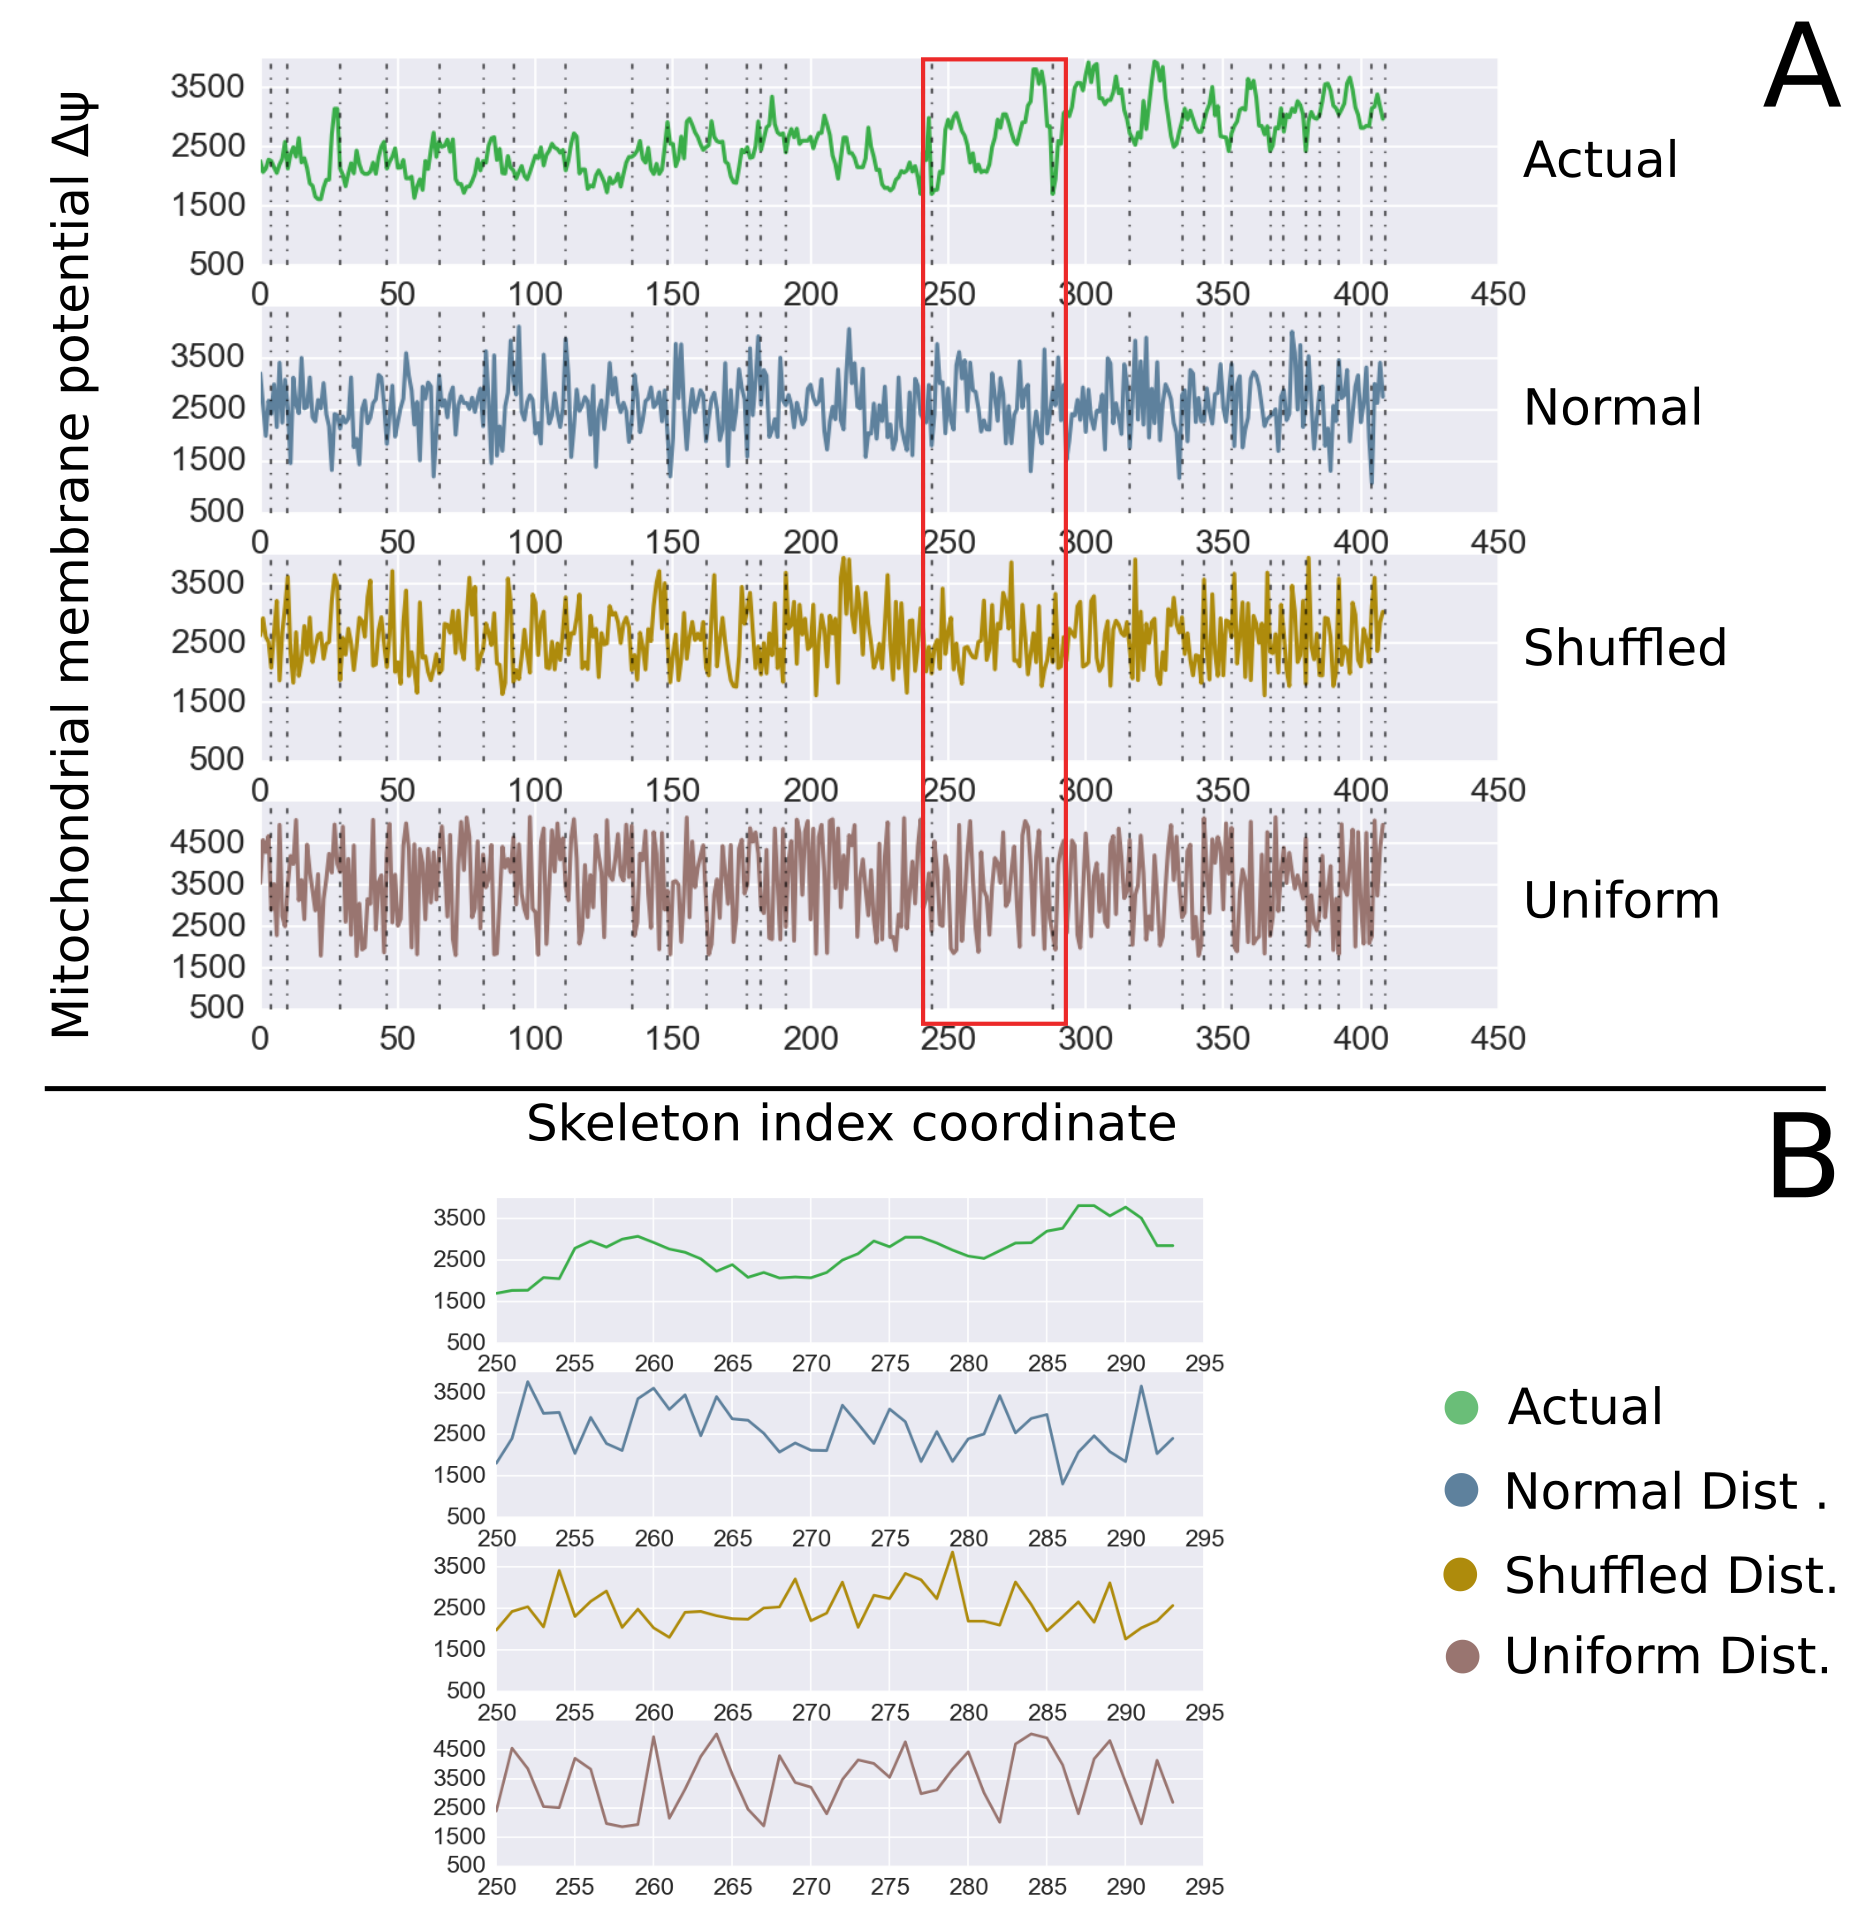
\includegraphics[width=.95\textwidth]{random}
    \subcaptionbox{ΔΨ distribution in all tubules from a single cell. The x-axis represents a coordinate system where all the tubules in that cell are lined up end to end. The vertical dotted lines indicate the boundaries of a tubule within that cell. The red box highlights a single tubule and is shown in more detail in the \Fref{fig:randomB}.\label{fig:randomA}}[\linewidth]{}
    \subcaptionbox{ΔΨ distribution in a single tubule from the same cell (highlighted by the red box in \Fref{fig:randomA}). \label{fig:randomB}}[\linewidth]{}
    \caption[Tubule level ΔΨ heterogeneity in actual and random distributions]{Tubule level ΔΨ heterogeneity in actual and random distributions.\\Mitochondrial membrane potential (ΔΨ) distribution in tubules are plotted and compared with fitted random distributions. The three random distributions below the 'Actual' distribution represent baseline levels of mitochondrial ΔΨ homogeneously distributed with random variations due to optical and experimental conditions. Actual distributions of ΔΨ display much smaller variation in ΔΨ between adjacent pixels.
}\label{fig:random}
\end{figure}
%
\subsection{Sampling of random distributions}
The random distributions shown in (\Fref{fig:random}) were obtained as follows:
For each cell, let the mitochondrial network with a total of $N$ pixels be a vector of signal intensities $\{X_0, X_1 \cdots X_{N-1}\}$, where the subscripts indicate the order indices of the pixels. The signal intensities represent the normalized ΔΨ as described in \Fref{ch:two}. The indices represent the coordinates of the pixels along an imaginary one dimensional axis that would be obtained from lining up all the tubules in the mitochondrial network end to end.

We calculate the sample mean and variance of this set, $\mu$ and $\sigma^2$ as follows:\\
At each pixel position, we sampled from a normal distribution $N(\mu,\sigma^2)$  to get sampled intensities $\{X_{s0}, X_{s1} \cdots X_{sN-1}\}$. This is was then plotted as the 'Normal' distribution graph shown in \Fref{fig:random}. A similar procedure was used for the 'Uniform' distribution graph, where we sampled from a uniform distribution $U(\mu-1.5\sigma, \mu+1.5\sigma)$ at each pixel position. The range of the uniform distribution was chosen so as to approximate a distribution that encompassed 99.7\% of the Normal distribution range.
For the 'Shuffled' distribution graph, we randomly permuted the set of original signal intensities to get a permuted set $\{X_{p0}, X_{p1}, \cdots X_{pN-1}\}$, where for example, the signal intensity $X_{p0}$ represents the randomly shuffled signal intensity at the pixel position 0.
\subsection{Autocorrelation curves}
The autocorrelation coefficient $R(k)$ measures the 'memory' of a signal by correlating pairs of points within the signal separated by a lag distance, $k$. A high value of autocorrelation at large lag distances implies that the signal has memory at large length scales.
The autocorrelation curves for \Fref{fig:autorandom} and \Fref{fig:autoactual} were derived as follows:
For a single tubule of length $N$ with signal intensity $\{X_0, X_1 \cdots X_{N-1}\}$ the autocorrelation coefficient $R(k)$ as a function of pixel lag distance $k$, was calculated as \cite{priestley1981spectral}:
\begin{align}\label{eq:autocor}
	R(k)&=\frac{1}{(N-k)\sigma^2} \, \displaystyle\sum_{t=1}^{N-k}  (X_t-\mu )( X_{t+k}-\mu) \nonumber \\
	&\! \text{for }k_0,k_1 \cdots k_{15}
\end{align}
The terms $\mu$ and $\sigma$ are the sample mean and variance of the tubule respectively. Since we are using the sample mean and variance, the autocorrelation coefficient is a biased estimate. We restricted our tubules to a minimum length of 40 pixels to minimize the bias error from using the sample mean and variance while ensuring we had enough tubules to obtain sufficient statistical power. For the populations of tubules from the various carbon source we had a range of 144--250 tubules with this minimum length (glucose=144, glycerol+ethanol=218, lactate=230, raffinose=177). This represented 10--15\% of the total tubule population. We then averaged all the autocorrelation coefficient at a given lag distance $k$ and plotted the mean autocorrelation curve for tubules with this minimum length. Tubules from populations of cells from random distributions (\Fref{fig:autorandom}) and growing in different carbon sources (\Fref{fig:autoactual}) were plotted.
%
\begin{figure}[htp]
	\centering
    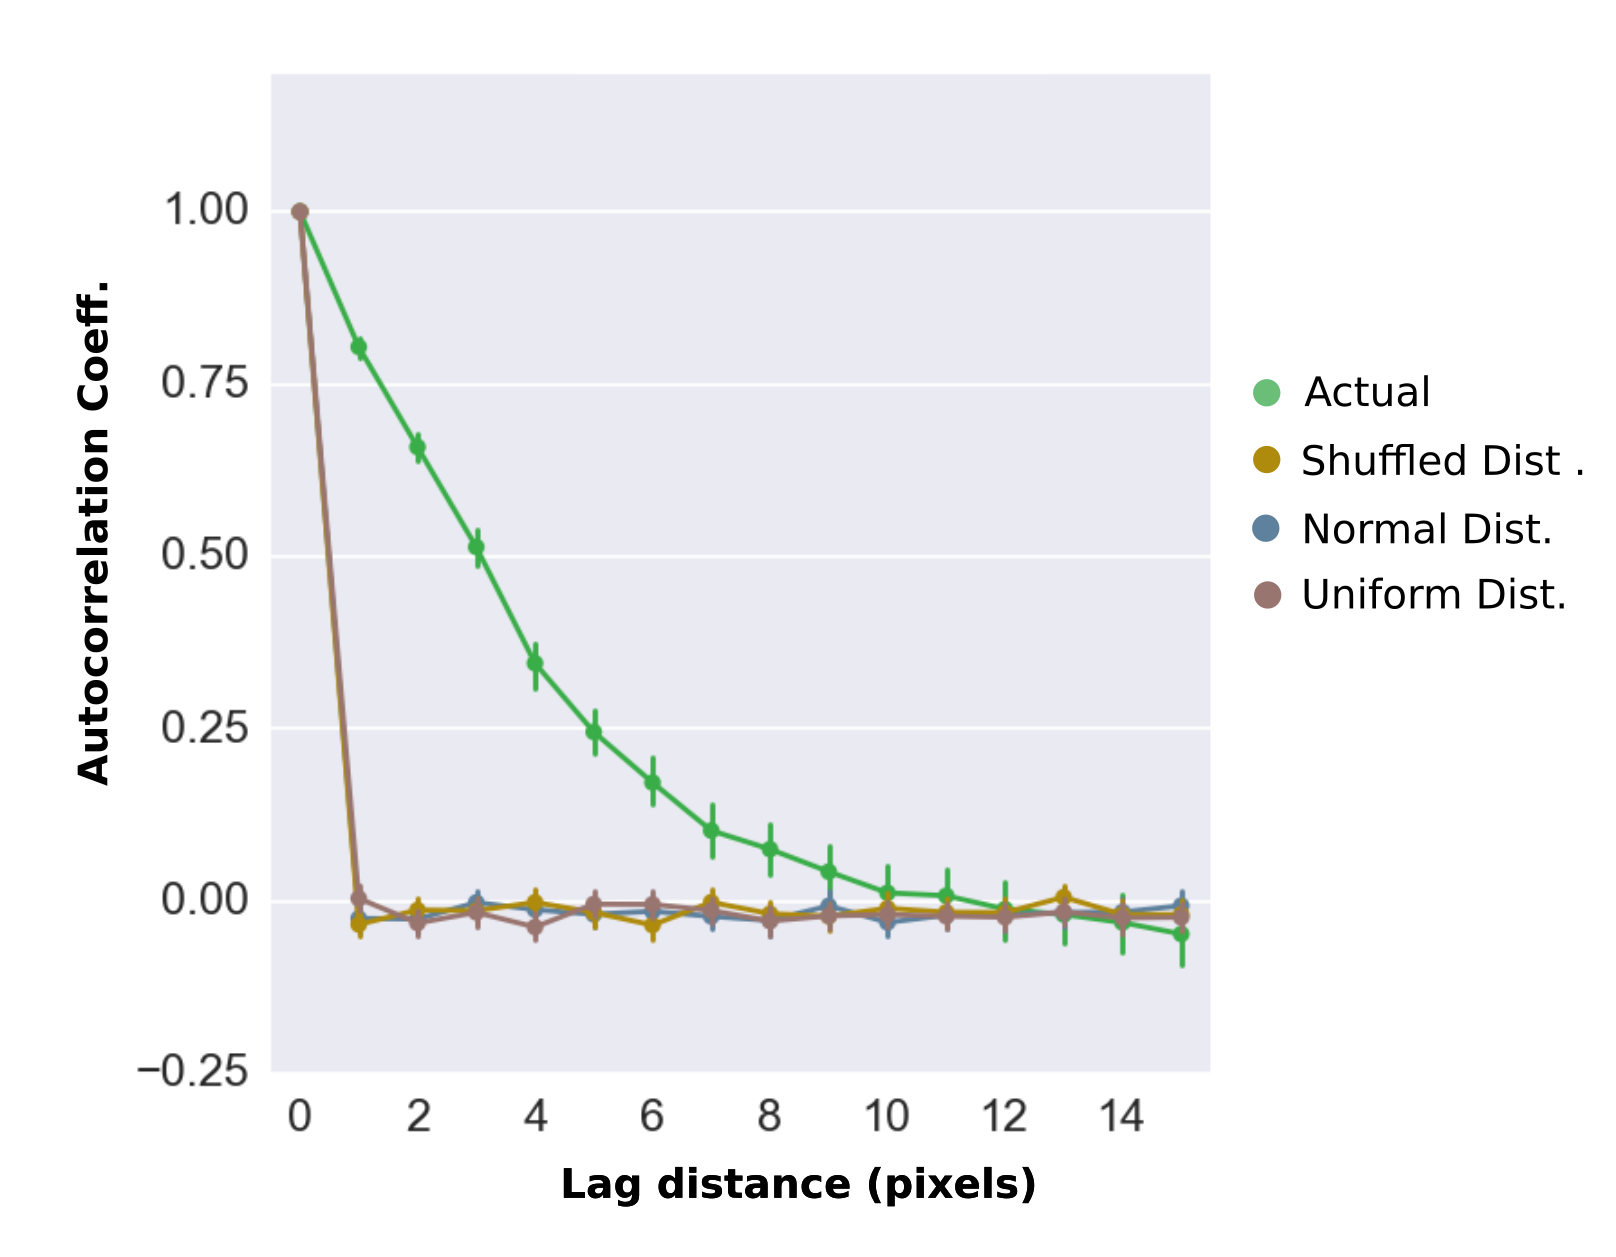
\includegraphics[width=.75\textwidth]{autorandom}
    \caption[Autocorrelation curves of actual vs random distributions]{Autocorrelation curves of actual vs random distributions.\\Shown here is the autocorrelation coefficient distribution of a real population of cells (green curve, grown in glycerol+ethanol) and three random populations. The autocorrelation of ΔΨ distribution from a real population of mitochondrial tubules displays higher autocorrelation coefficients at large length scales (lag distance) compared to random distributions.\\\emph{Error bars represent the bootstrapped 95\% confidence interval of the mean.}}\label{fig:autorandom}
\end{figure}
%
%
\begin{figure}[htp]
	\centering
    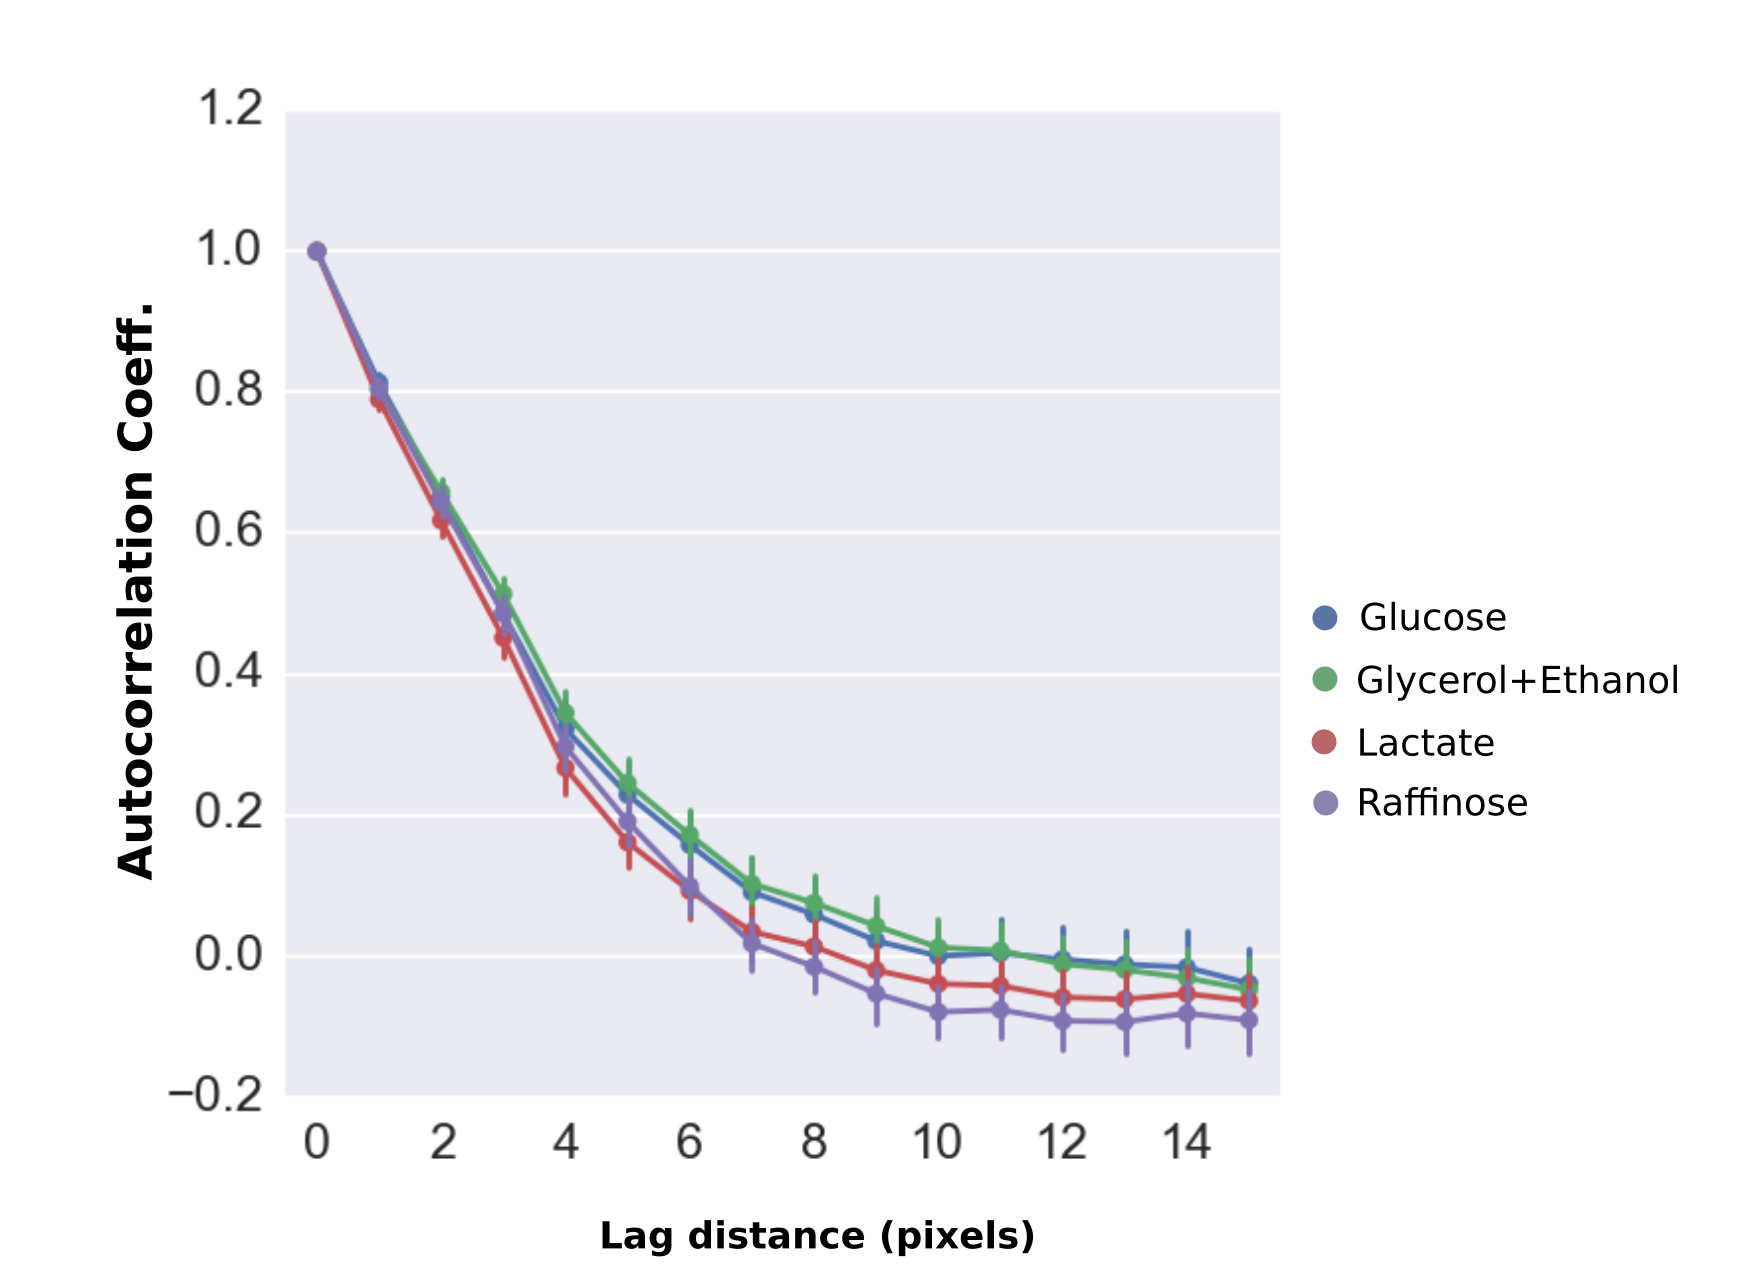
\includegraphics[width=.7\textwidth]{autoactual}
    \caption[Autocorrelation curves of populations of cells growing in different carbon sources]{Autocorrelation curves of populations of cells growing in different carbon sources .\\Shown here are the autocorrelation coefficient distributions of cells grown in either fermentation (glucose), respiration only (glycerol+ethanol, lactate) and respiration+fermentation (raffinose). Mitochondrial tubules grown in the different conditions do not show a statistical difference in their autocorrelation curves.\\\emph{Error bars represent the bootstrapped 95\% confidence interval of the mean.}}\label{fig:autoactual}
\end{figure}
%
%
\begin{figure}[htp]
	\centering
    \hspace*{.65in}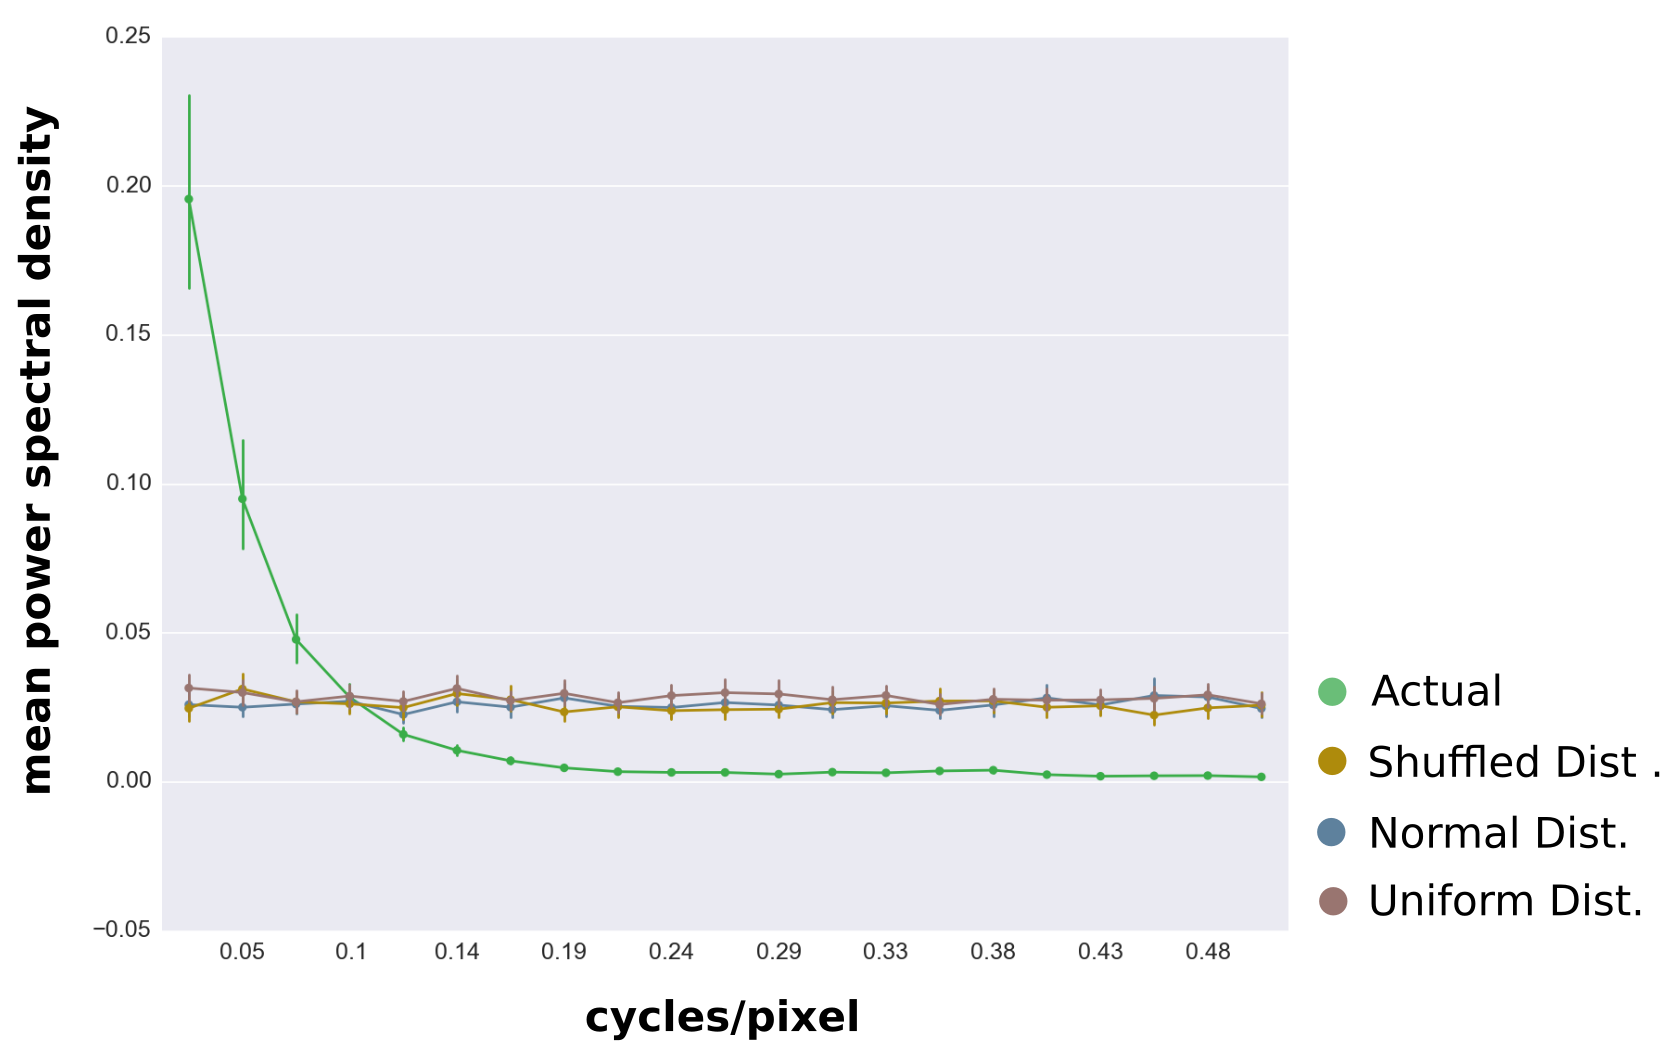
\includegraphics[width=.8\textwidth]{psdrandom}
    \caption[Power spectral density of actual vs random distributions]{Power spectral density of actual vs random distributions.\\Shown here is the power spectral density of a real population of cells (green curve, grown in glycerol+ethanol) and three random populations. The power spectral density of ΔΨ from a real population of mitochondrial tubules displays much more power at lower spatial frequencies (i.e. higher correlation at larger length scales) compared to random distributions (observe the high power on the y-axis at values of <0.1 for the x-axis compared to the random distributions).\\\emph{Error bars represent the bootstrapped 95\% confidence interval of the mean.}}\label{fig:psdrandom}
\end{figure}
%
%
\begin{figure}[htp]
	\centering
    \hspace*{.65in}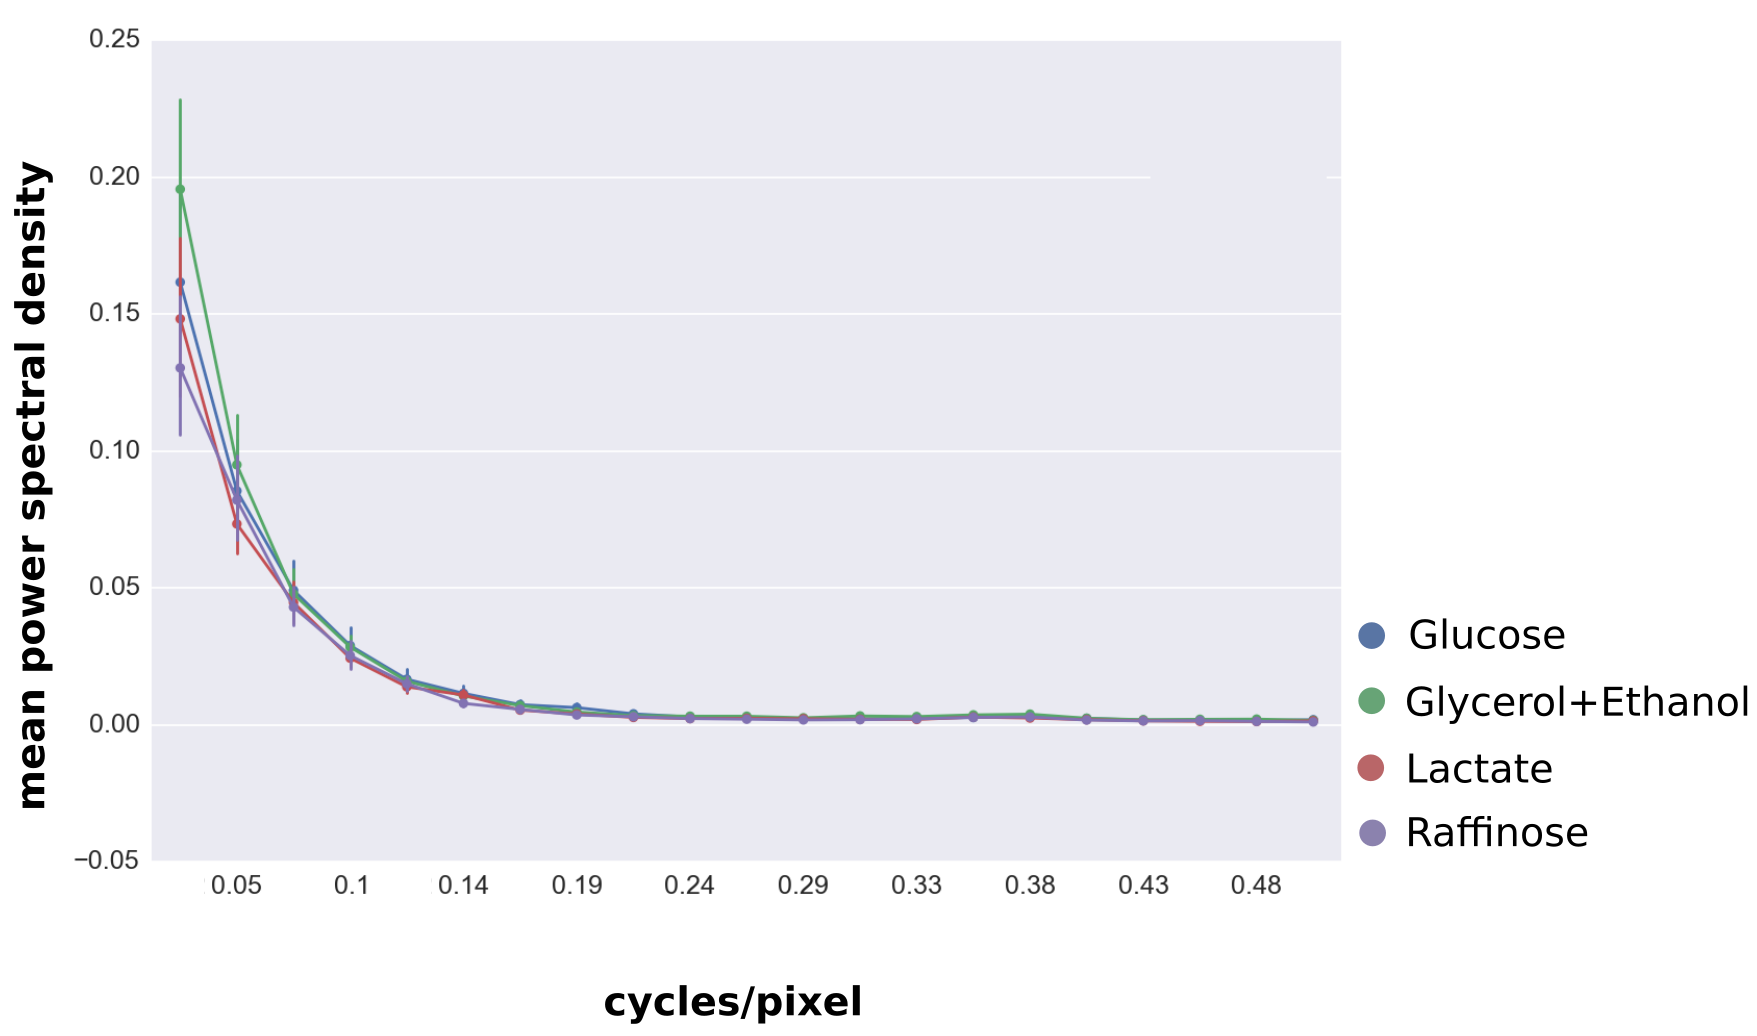
\includegraphics[width=.85\textwidth]{psdactual}
    \caption[Power spectral density of populations of cells growing in different carbon sources]{Power spectral density of populations of cells growing in different carbon sources.\\Shown here are the power spectral densities of cells grown in either fermentation (glucose), respiration only (glycerol+ethanol, lactate) and respiration+fermentation (raffinose). Mitochondrial tubules grown in respiration and fermentation (glucose) do not show a statistical difference in their spatial frequency content.\\\emph{Error bars represent the bootstrapped 95\% confidence interval of the mean.}}\label{fig:psdactual}
\end{figure}
%
\subsection{Power spectral density}
The power spectral density (PSD) is defined as the square of the modulus of the Fourier transform of a signal and is a measure of the spatial frequency content of the signal. Spatial frequency is the inverse of spatial length, a higher spatial frequency implies a smaller length scale \cite{schowengerdt_chapter_2007}. For a single tubule of length $N$ with signal intensity $\{X_0, X_1 \cdots X_{N-1}\}$ and sampling rate of $Δt=1$ pixel, the power spectral density $S(f)$ as a function of spatial frequency $f$ is estimated as the modulus squared of the discrete Fourier transform (DFT) \cite{priestley1981spectral}:
\begin{align}
	S(f)&=\frac{Δt}{N} \: \left\vert\displaystyle\sum_{t=0}^{N-1}  X_n \exp ^{-i 2 \pi nf}\right\vert^2 \nonumber \\
	&\! f\leq \frac{1}{2Δt} \; \text{for real frequencies}
\end{align}

We calculated the power spectral density using the Numpy.fft.rfft module (\url{http://www.numpy.org/}), which calculates the DFT for real input functions. Since we are limited to a sampling resolution of 1 pixel, the maximum frequency we can get will be 0.5 cycles/per pixel. Ideally $N$ should be as large as possible to get the 'true PSD', i.e. with larger $N$ we will get finer resolutions of $S(f)$. Similar to the derivation of the autocorrelation curve, we restricted our tubules population to be a minimum of length 40 pixels so that we get a minimum of 20 values of $f$ between 0--0.5 cycles/pixel. The DFT returns positive and negative frequencies; we ignore negative frequencies for real spatial values. We then averaged the function by spatial frequency $f$ and plotted the mean $S(f)$ curve for all the tubules in the population. Tubule populations of cells from random distributions and in different growth conditions were plotted (\Fref{fig:psdrandom} and \Fref{fig:psdactual}).

By the Wiener–Khinchin theorem \cite{kay1981spectrum}, the power spectral density $S(f)$ is the Fourier transform of the autocorrelation function $R(k)$:
\begin{equation}
	S(f)= \displaystyle\sum_{k=-\infty}^{\infty} R(k) \exp^{-i 2 \pi n f}
\end{equation}
Therefore we can think of the power spectral density as the frequency transformed version of the information provided by the autocorrelation curves. A power spectrum that has high power at low frequencies implies a greater correlation at large length scales. 
\subsection{Delta intensity \texorpdfstring{$ΔI(k)$}{DIk}}
One problem with using autocorrelation is that we are using a biased estimate of the autocorrelation due to using the sample mean and variance of the tubule. Therefore in order to minimize the sample bias we restricted the tubule population to a minimum length 40 pixels, but this meant we were excluding a large proportion of tubules that fell below this threshold (up to 90\% of the tubules).
Referring to \eqref{eq:autocor}, the terms inside the summation represent the covariance between points on the tubule. Instead of using the covariance, we defined another function $ΔI(k)$:
\begin{align}
	ΔI(k)&= \left\vert \displaystyle\sum_{t=1}^{N-k} X_t-X_{t+k} \right\vert \nonumber \\
	& \! \text{for }k_1,k_5,k_{10},k_{15},k_{20}
\end{align}
%
\begin{figure}[htp]
	\centering
    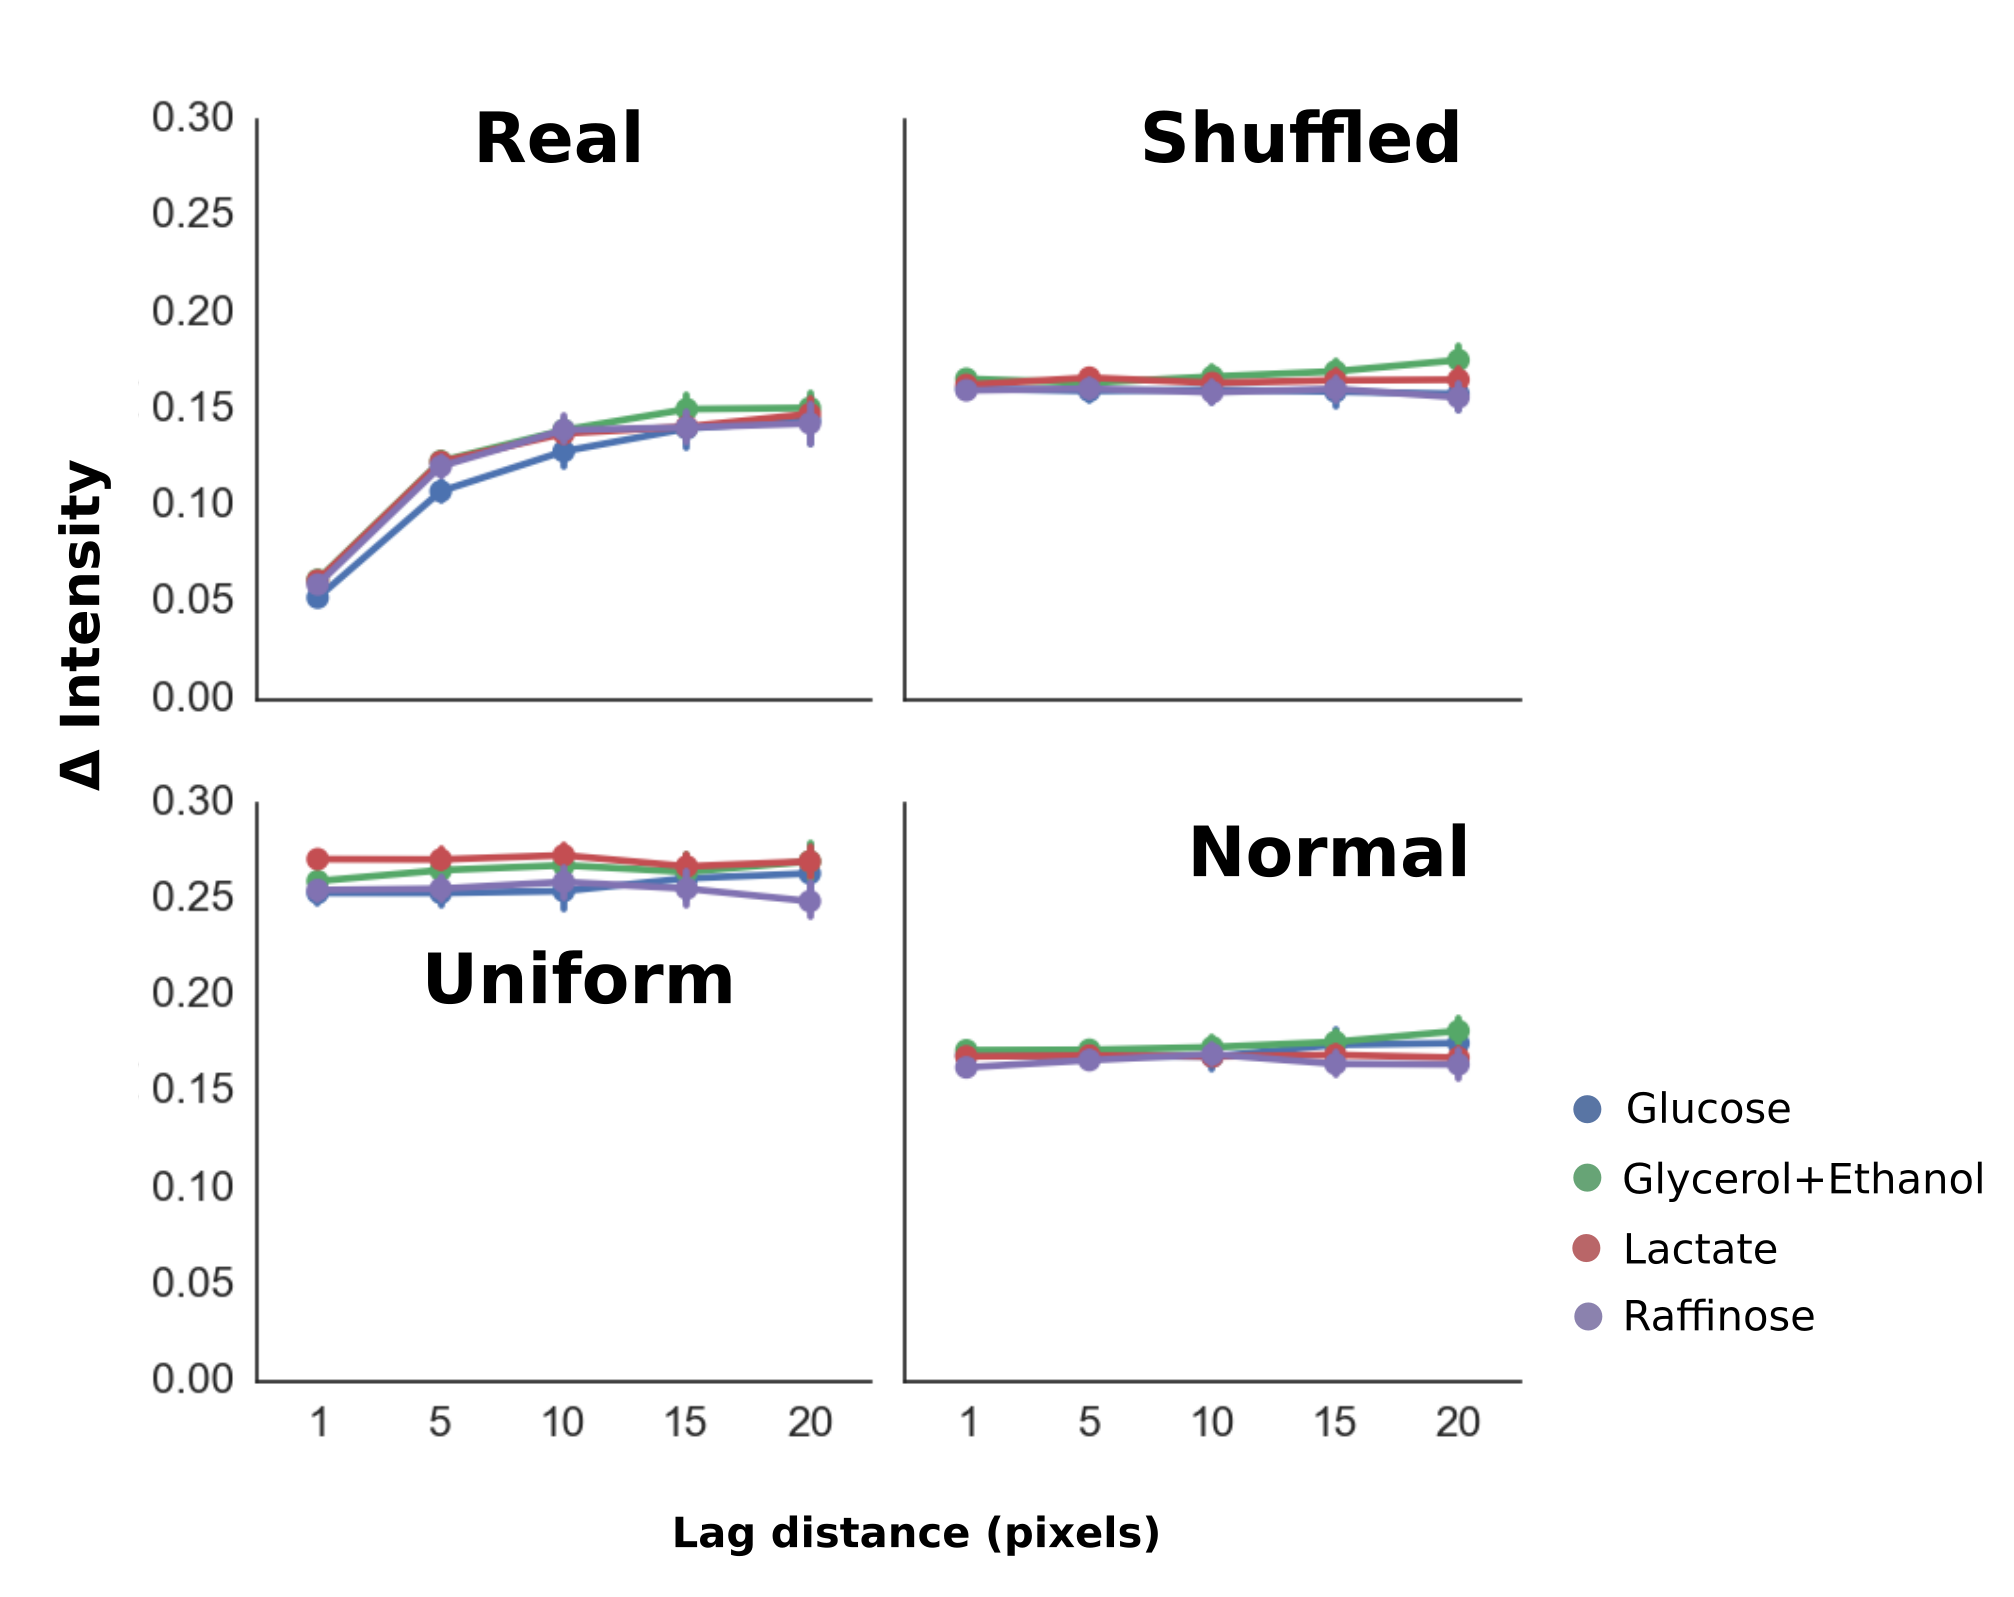
\includegraphics[width=\textwidth]{deltaI}
    \caption[Delta intensity $ΔI(k)$ curves]{Actual and random delta intensity ($ΔI(k)$) curves.\\The plot shows a panel of delta intensity $ΔI(k)$ distributions for the populations of cells grown in different carbon sources. The top left pane shows the $ΔI(k)$ of the actual populations of mitochondrial tubules grown in different carbon sources. The top right and bottom panels show the $ΔI(k)$ distribution of the random distributions (Shuffled, Uniform, Normal) plotted for each of the carbon sources. Mitochondrial tubules in all of the different carbon sources show non random distribution of $ΔI(k)$.\\\emph{Error bars represent the bootstrapped 95\% confidence interval of the mean.}}\label{fig:deltaI}
\end{figure}
%
%
\begin{figure}[htp]
	\centering
    \hspace*{.7in}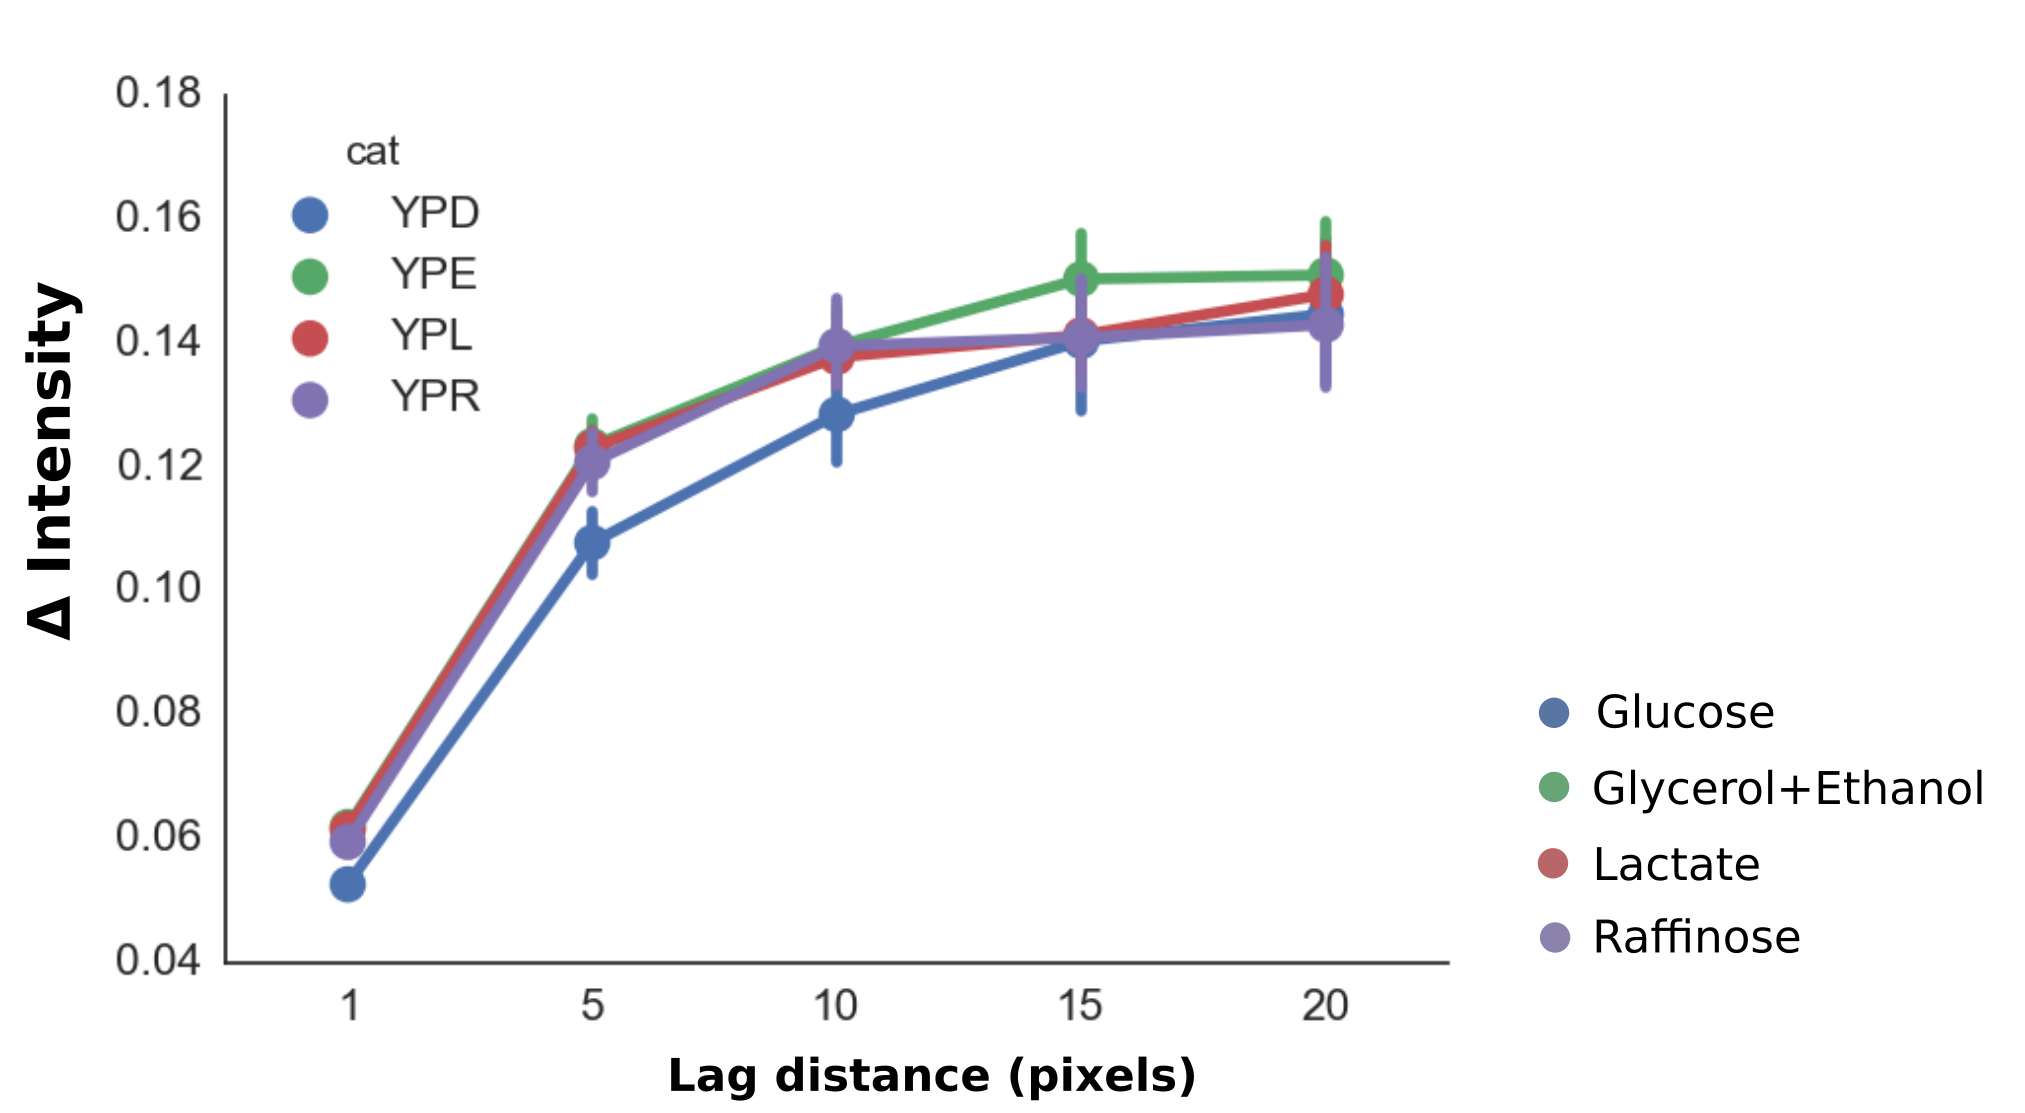
\includegraphics[width=.85\textwidth]{deltaIactual}
    \caption[$ΔI(k)$ actual for tubule populations growing in different carbon sources]{$ΔI(k)$ actual for tubule populations growing in different carbon sources.\\Mitochondrial tubules in fermentation (glucose) have lower $ΔI(k)$ at lag distances below 15 pixels, meaning that they show lower spatial frequencies and higher correlations at large length scales compared to respiratory conditions.\\\emph{Error bars represent the bootstrapped 95\% confidence interval of the mean.}}\label{fig:deltaIactual}
\end{figure}
%
This function represents the absolute difference of intensities between a pixel and another pixel separated by lag distance $k$. A large value of $ΔI(k)$ at small lag distances $k$ indicates that there is little correlation between those two pixels, and a high spatial frequency component to the signal. We averaged the function at a given lag distance $k$ and plotted the mean $ΔI(k)$ curve for all the tubules in the population. Tubule populations of cells from random distributions and in different growth conditions were plotted (\Fref{fig:deltaI} and \Fref{fig:deltaIactual}).
 
\subsection{Statistical testing with post-hoc multiple testing correction}\label{sec:stat}
In this project, whenever we made a statistical test comparing two conditions we used the ranked sum test with $p<0.05$ as the significance level to reject the null hypothesis that there was no difference between the two conditions. When performing statistical testing across multiple conditions, there is an increasing probability of making a false positive (Type I error) across all tests. This probability is known as the family wise error rate (FWER) and is given by the formula:
\begin{equation}
	\text{FWER}=1-(1-p)^n
\end{equation}
$p$ is the significance level for one comparison and $n$ is the number of comparisons. For our project, with four different carbon conditions there are six possible combinations, and at a typical significance level where we reject the null hypothesis of $p=0.05$, the FWER is \textasciitilde{27\%}. Thus it is critical that all statistical tests be corrected for multiple testing with a post-hoc correction method. We used the Holms-Sidak \cite{holm_simple_1979} multiple testing correction method which has been shown to have more statistical power \cite{seaman_new_1991} (i.e. more likely to detect an effect if the effect really existed) than the popular Tukey or Bonferonni methods while ensuring that the FWER is less than 0.05 (thus avoiding false positives due to multiple testing). The Holms-Sidak method is a recursive step-down method where the $p$ values are ranked and compared with successively larger adjusted significance levels. The method is guaranteed to control the FWER which we set at 0.05, but the disadvantage is that we cannot obtain the confidence intervals from the test. We do not require a confidence interval in our analysis for this chapter as we are only interested in whether there is a difference between the groups.

The above procedure was carried out using the StatsModels package in Python (\url{http://statsmodels.sourceforge.net/devel/generated/statsmodels.sandbox.stats.multicomp.multipletests.html}).
\section{Results}
\subsection{Mitochondrial tubules have nonrandom heterogeneity of ΔΨ}
In order to conclusively determine whether heterogeneity of ΔΨ exists within mitochondrial tubules, we must first establish a baseline to decide if a ΔΨ distribution is truly heterogeneous. We do this by comparing the distributions of the signal intensities to random distributions of ΔΨ intensities. In \Fref{fig:random} we show three different types of random distributions ('Normal, Shuffled, Uniform') below an actual distribution of ΔΨ. These three random distributions represent a 'control' or baseline level of ΔΨ homogeneously distributed with random variations due noise in the optics and experimental conditions. The Shuffled distribution is the most conservative estimate of a true random baseline as it is non parametric and does not need any estimation of the distribution parameters. The Normal distribution represents a random distribution of ΔΨ that would be observed with a Gaussian uptake level of the ΔΨ dye. The Uniform distribution represents uniformly constant dye uptake and variances due to optical and experimental setup.

The observed actual distribution differs from the random networks of ΔΨ intensities as they show smaller variations in intensities between adjacent pixel positions (\Fref{fig:randomB}). In order to quantify this difference between actual and random distributions, we calculated the autocorrelation, power spectral density and delta intensity curves for the population of tubules of actual and random distributions using the methods described in \fref{sec:mmch4}. 

As shown in \Fref{fig:autorandom} the correlations of ΔΨ intensities in actual tubule distributions decay much slower than random networks, i.e. they are correlated over larger length scales. This is also shown in \Fref{fig:psdrandom}, where the spectrum of the random distributions is much more 'spread out' compared to real distributions, i.e. they have higher powers at higher spatial frequencies. The crossover point for the spectrum of real and random distributions is around 0.1 cycles/pixel, i.e. real networks do not seem to have much correlations in their signal intensities beyond length scales >10 pixels.

Similar behavior is exhibited in \Fref{fig:deltaI}, where the random distributions exhibit much larger change in their $ΔI(k)$ at small lag distances and that real distributions effectively become random at lag distances \textasciitilde{10} pixels (compare 'real' to 'shuffled' in \Fref{fig:deltaI}).
\subsection{Mitochondrial tubules in respiratory conditions have less correlation of ΔΨ at large length scales compared to fermentative conditions}\label{sec:432}
The existence of heterogeneity within a mitochondrial tubule leads us to ask if this heterogeneity is affected by the bioenergetic state of the cell. Previous studies have shown that OXPHOS proteins and cristae numbers are upregulated in mitochondria when respiration demand increases \cite{jimenez_mitochondrial_2014,mannella_relevance_2006}. These changes to the ultrastructure have the potential to affect the heterogeneity of ΔΨ within the tubule. In order to determine how ΔΨ heterogeneity was affected by the functional state of the mitochondria, we compared the heterogeneity of ΔΨ between cell populations grown in different carbon sources. Yeast were grown aerobically and under exponential growth in four different carbon sources - glucose, glycerol+ethanol, lactate and raffinose (details in \fref{sec:carbon}).
%
\begin{figure}[htp]
	\centering
    \hspace*{.7in}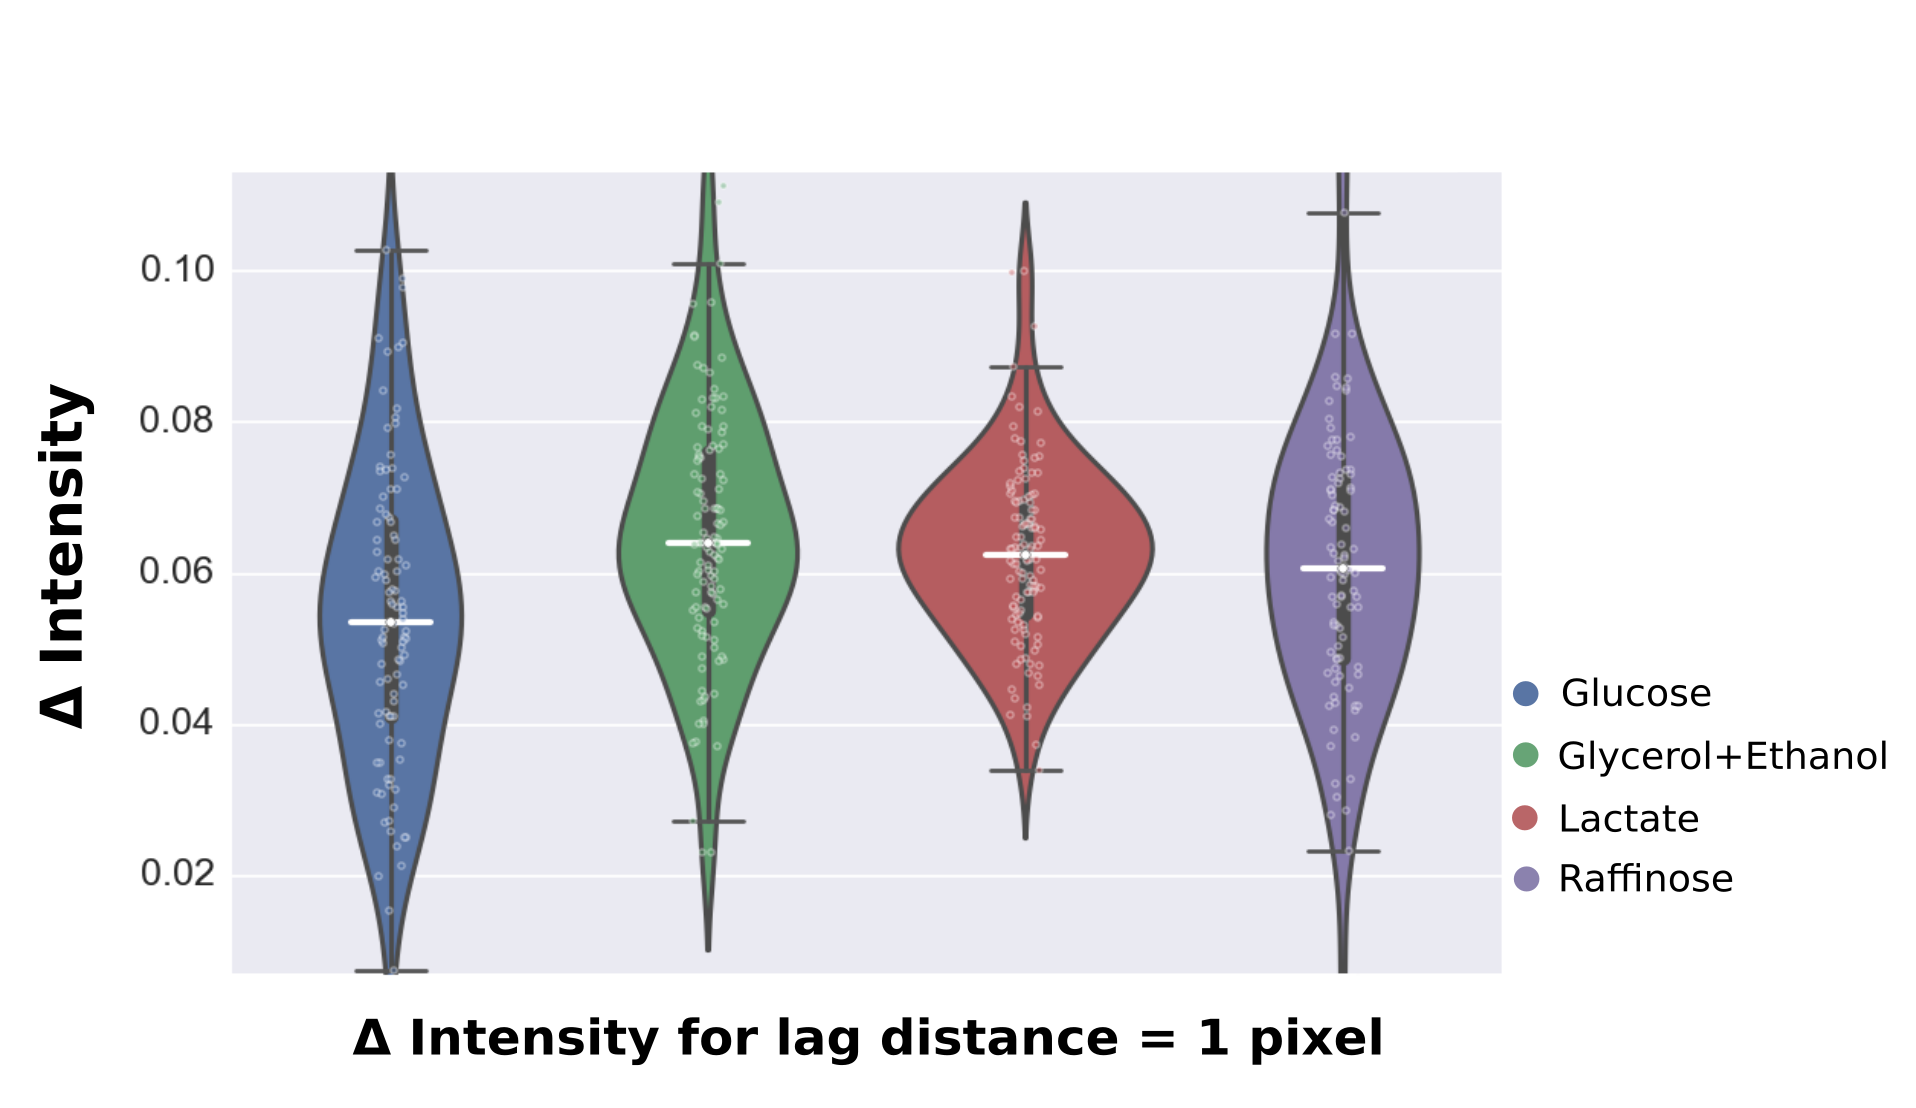
\includegraphics[width=.85\textwidth]{deltaIk1}
    \caption[Distribution for $ΔI(k=1)$]{Distribution for $ΔI(k=1)$.\\Violin plots for the distributions of $ΔI(k)$ in tubules, showing that there is a statistically significant lower value of $ΔI(k)$ at small lag distances for glucose, compared to the other three conditions which undergo respiration. Mitochondrial tubules grown in glucose have less power at high spatial frequencies.\\\emph{White bars indicate the median for the population.}}\label{fig:deltaIk1}
\end{figure}
%

We did not find a statistically significant difference in the autocorrelation curves or power spectral densities of the different growth conditions (\Fref{fig:autoactual} and \Fref{fig:psdactual}). This is evidenced by the fact that the confidence intervals indicated by the error bars overlap between the different populations.
This was surprising because we expect to see a difference between the respiratory (non glucose) and fermentative (glucose) conditions, as previously reported \cite{jimenez_mitochondrial_2014}. However it must be noted that the autocorrelation/power spectral density measures suffer from the fact that we clustered the tubules according to their lengths and it is difficult to compare all the tubules in a cell/population. The $ΔI(k)$ function (\Fref{fig:deltaIactual}) is able to obtain a more complete picture of tubule level heterogeneity across a wider range of tubule lengths. Using this method, we find a difference in heterogeneity characteristics between respiration and fermentation populations. Respiratory conditions have higher spatial frequencies and have less correlations at large length scales compared to fermentative conditions. This is evident in (\Fref{fig:deltaIk1}), where we plot the distributions of $ΔI(k=1)$. There is a statistically significant difference in the mean $ΔI(k=1)$ value between respiratory (non glucose) and fermentative (glucose) conditions (statistical test procedure done as in \fref{sec:stat}). Fermentative condition tubules have lower spatial frequencies and are more correlated over large length scales. They also seem to approach random distribution heterogeneity at a slower rate compared to respiratory tubules.
\subsection{Mitochondrial tubules in respiratory conditions have thicker width and more uniform distribution of thickness compared to fermentative conditions}
%
\begin{figure}[htp]
	\centering
    \hspace*{.5in}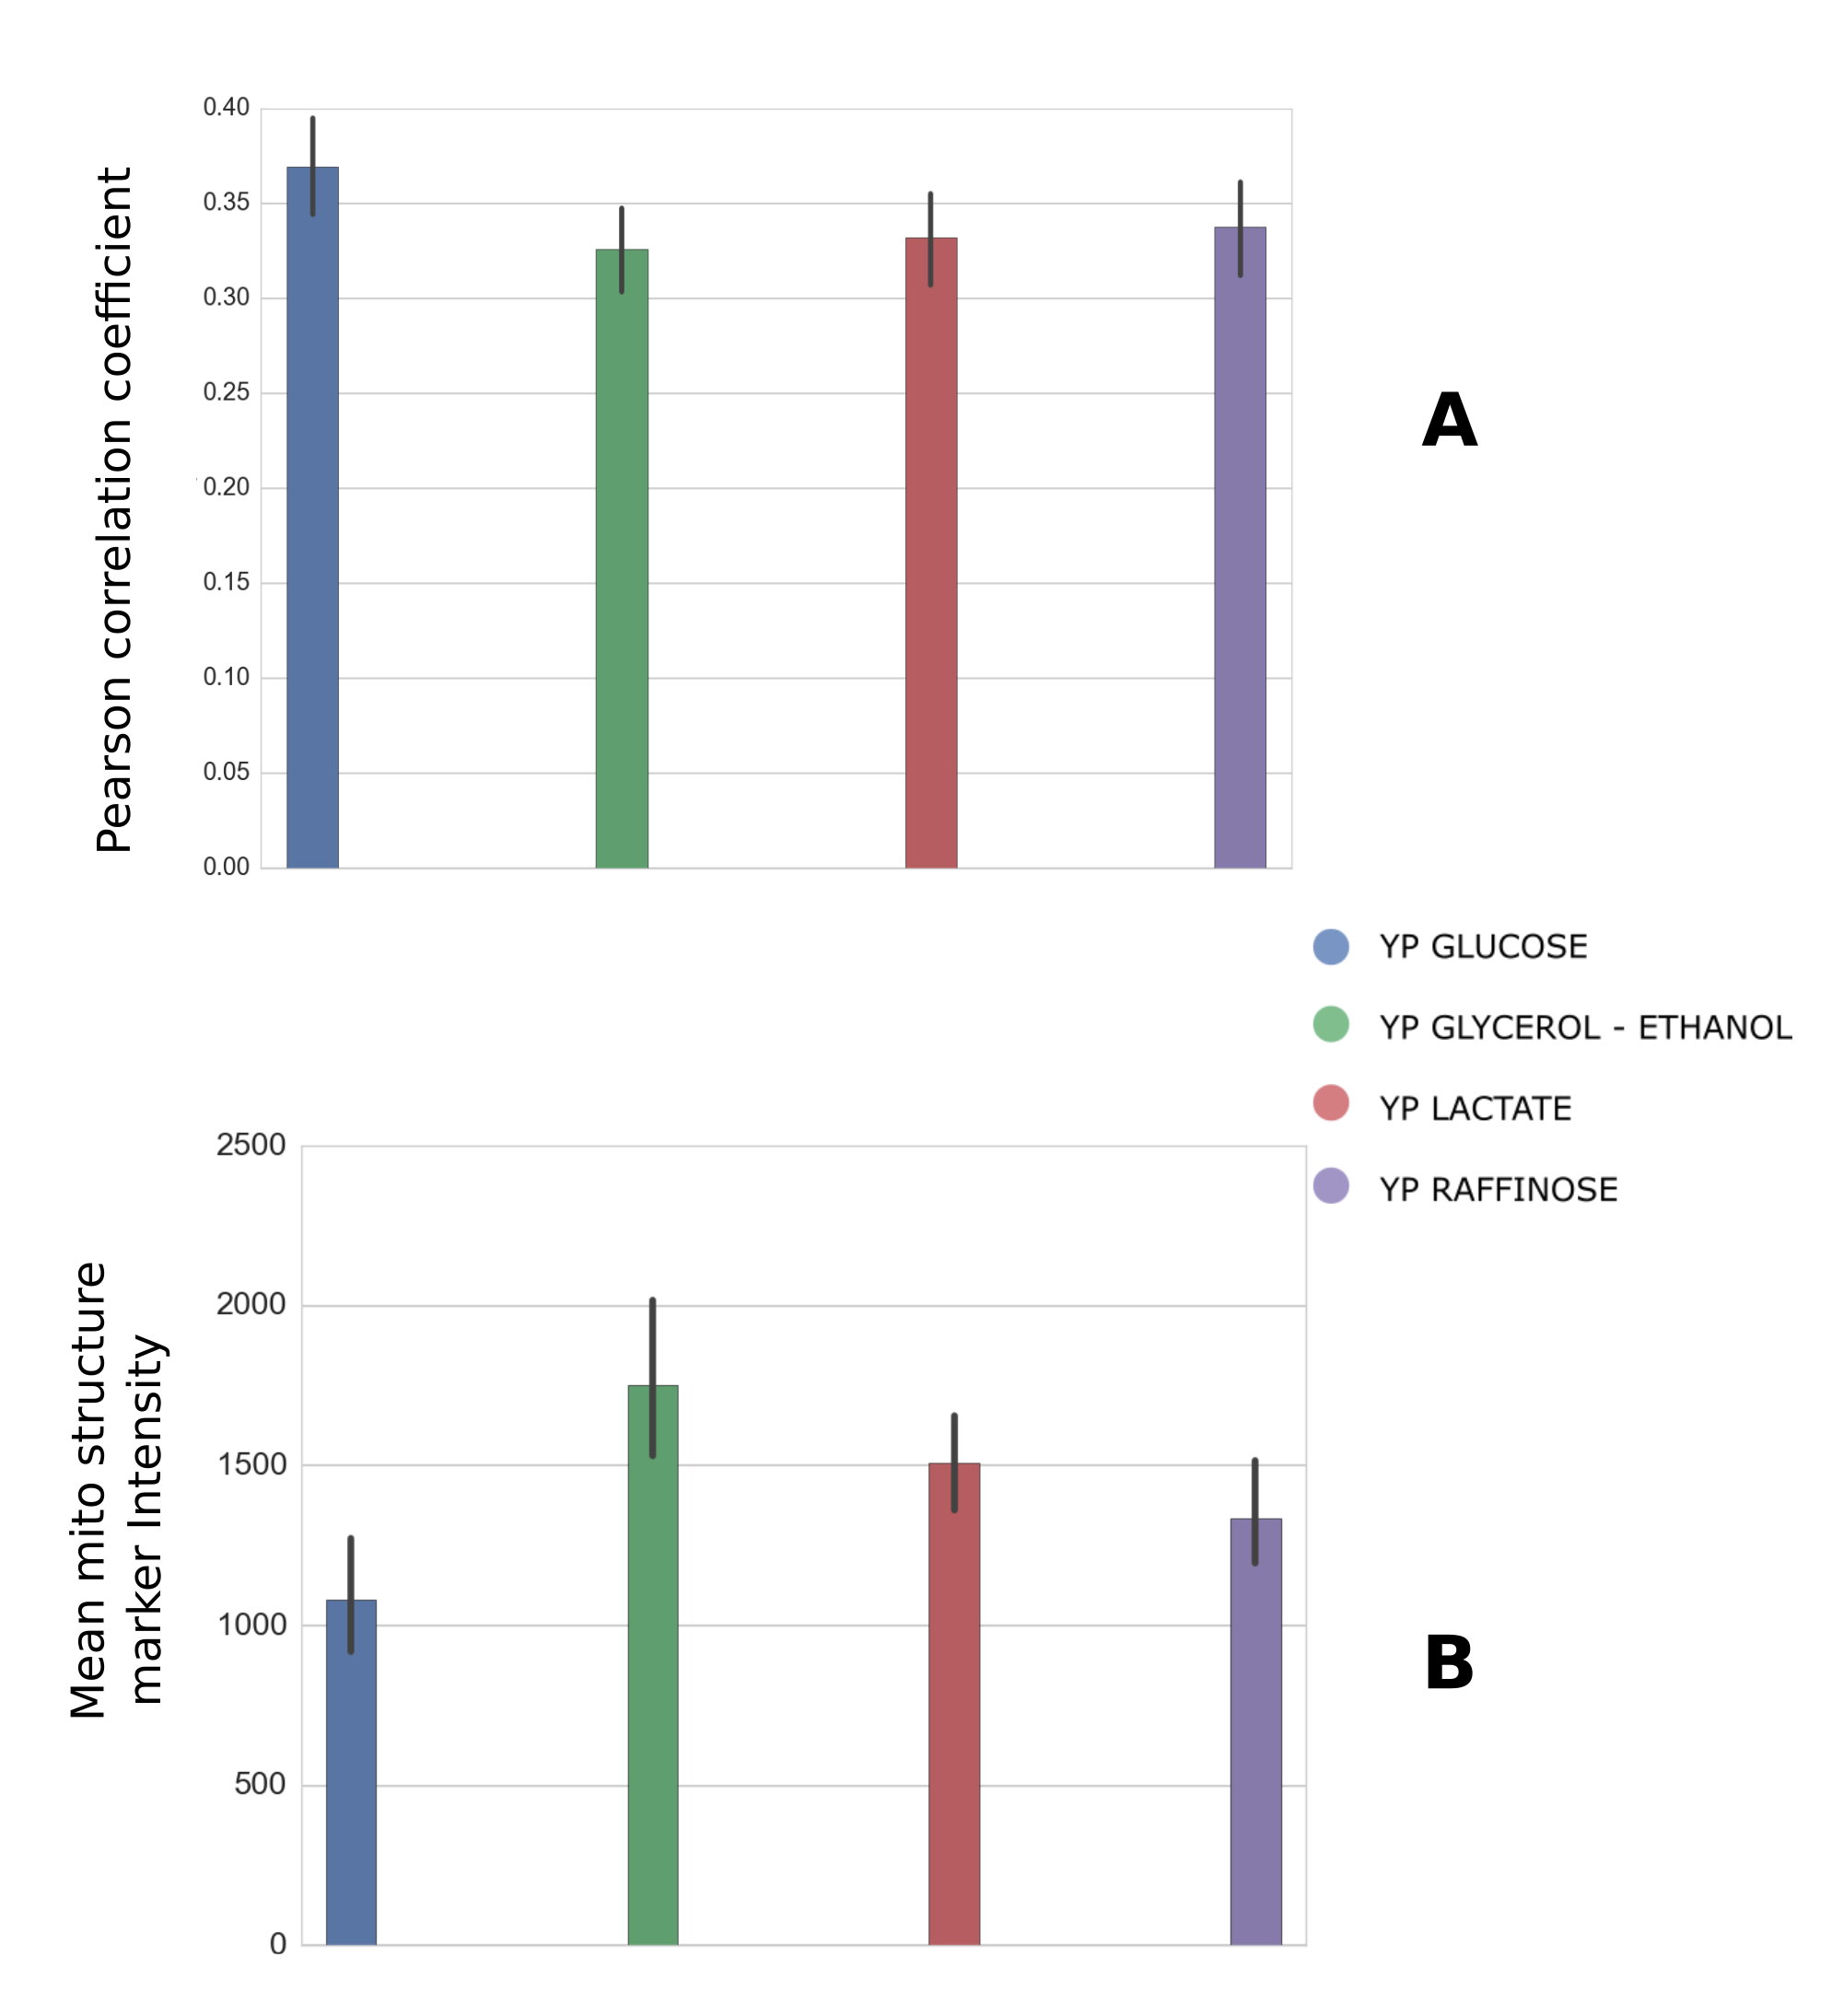
\includegraphics[width=.85\textwidth]{tubecontrol}
    \subcaptionbox{The Pearson correlation $R$ values between mitochondrial matrix marker intensity and tubule thickness show a mean value of \textasciitilde{0.35} for all the carbon conditions.\label{fig:tubecontrolA}}[\linewidth]{}
    \subcaptionbox{The variation between average (per cell) matrix marker intensity between the cells grown in different respiration conditions (non-glucose) show a large, statistically significant difference compared to the average tubule thickness shown in (\Fref{fig:tubewidth}). \label{fig:tubecontrolB}}[\linewidth]{}
    \caption[Tubule thickness variation is not an artifact of matrix intensities]{Tubule thickness variation is not an artifact of matrix intensities.\\Mitochondrial matrix marker intensities do not show strong correlation with tubule thickness (\Fref{fig:tubecontrolA}). The variation in matrix intensity is also much higher than the variation in tubule thickness (\Fref{fig:tubecontrolB}). Therefore measurements of tubule thickness derived from MitoGraph v2.0 are likely not affected by variations in matrix marker intensities.\\\emph{Error bars represent the bootstrapped 95\% confidence interval of the mean.}
}\label{fig:tubecontrol}
\end{figure}
%
%
\begin{figure}[htp]
	\centering
    \hspace*{.75in}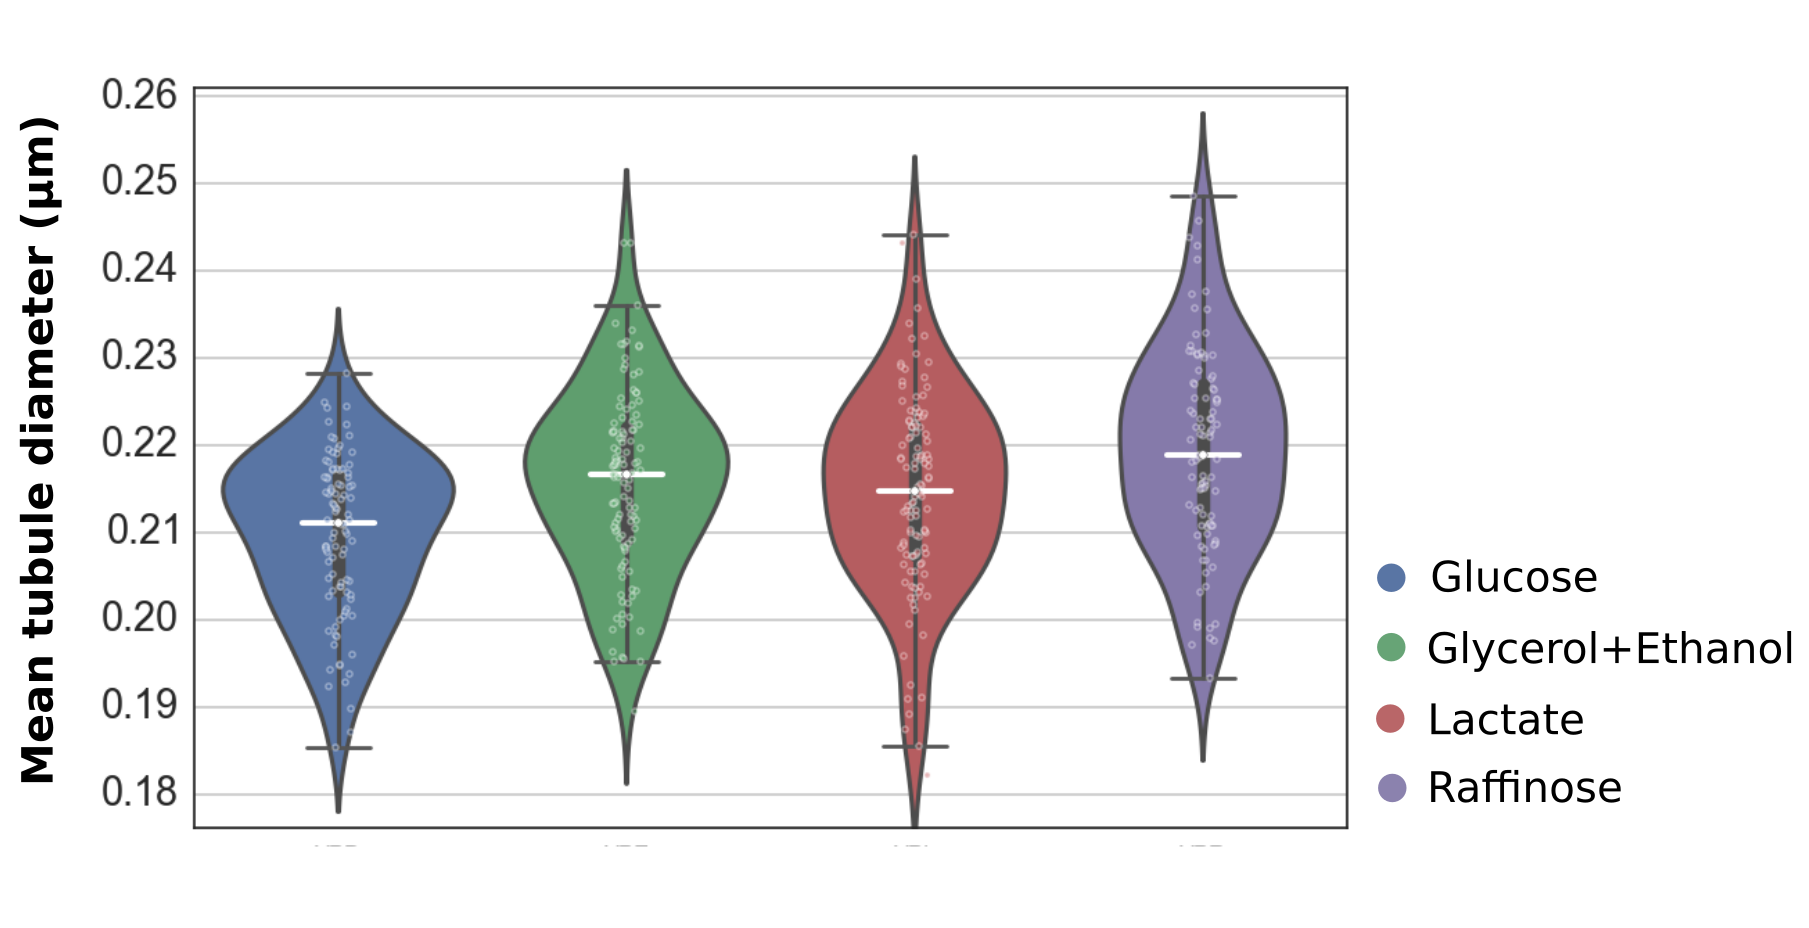
\includegraphics[width=.85\textwidth]{tubewidth}
    \caption[Distribution of mean tubule diameter per cell per population]{Distribution of mean tubule diameter per cell per population.\\The mean tubule diameters in respiration (non glucose) are statistically greater than the tubules in fermentation. The tubules are on average 2.6\% greater than in glucose.\\\emph{White bars indicate the median value.}}\label{fig:tubewidth}
\end{figure}
%
%
\begin{figure}[htp]
	\centering
    \hspace*{.5in}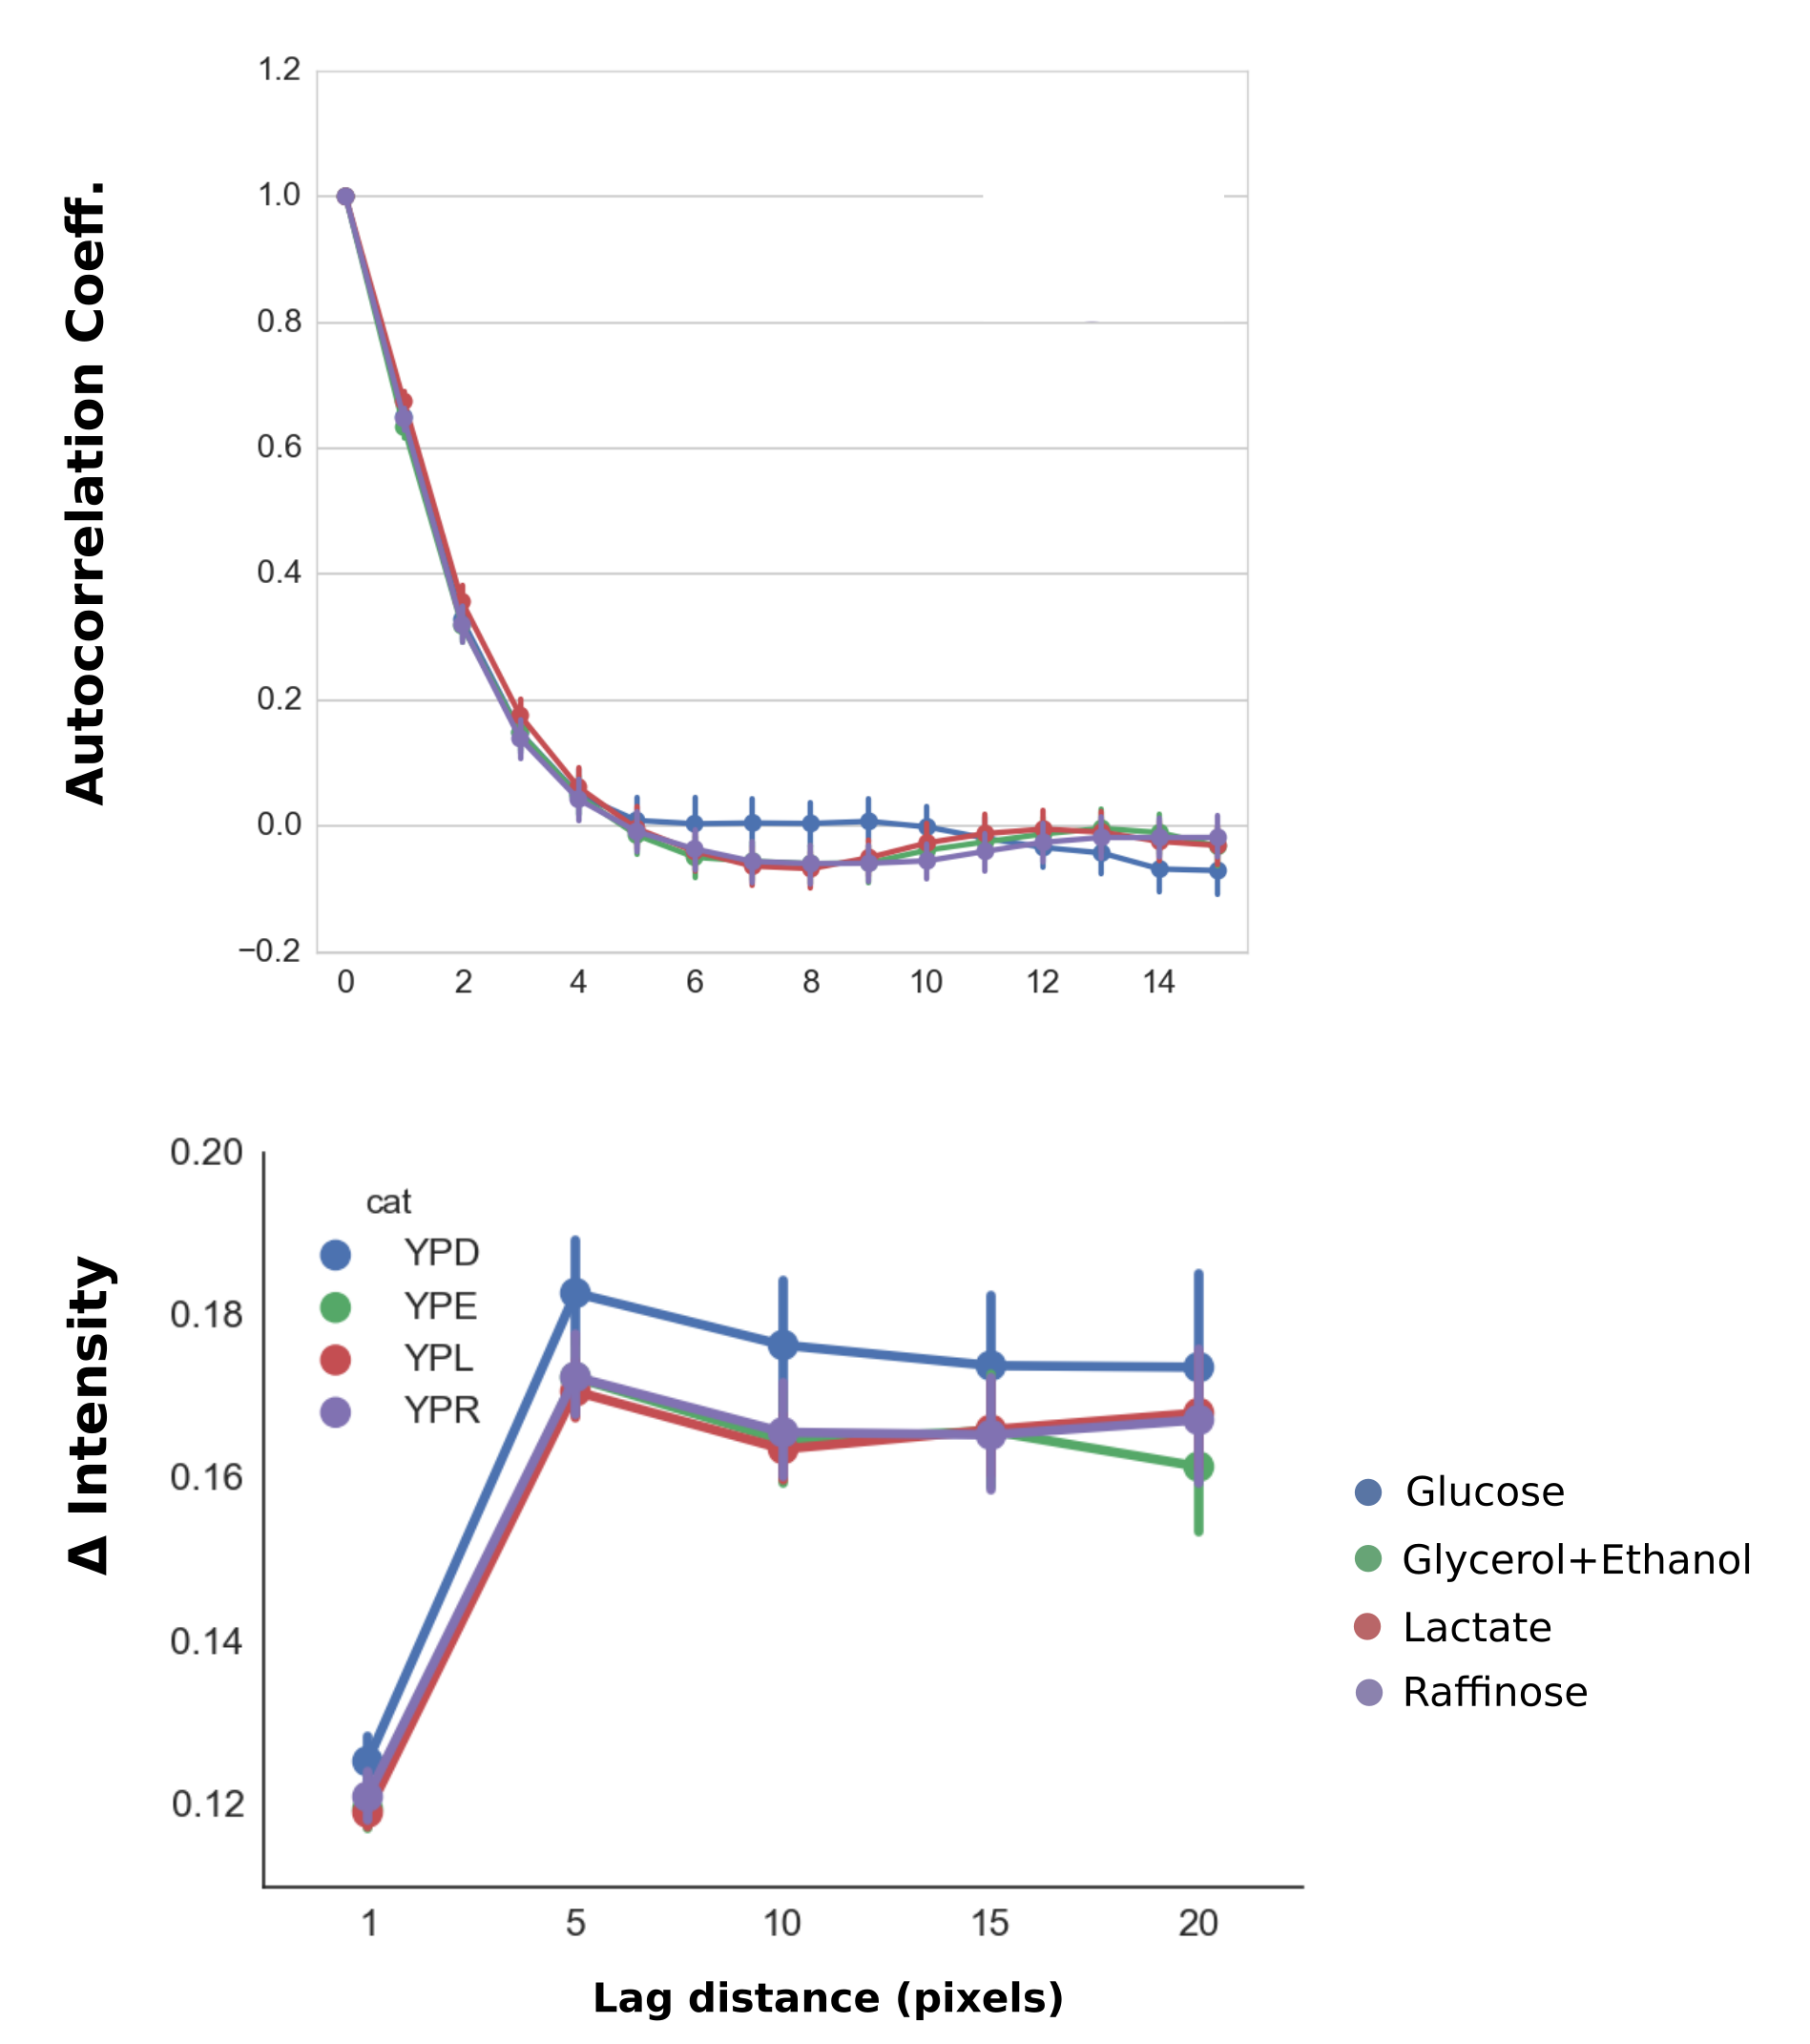
\includegraphics[width=.85\textwidth]{tubewidedist}
    \caption[Autocorrelation and $ΔI(k)$ curves of tubule diameter heterogeneity]{Autocorrelation and $ΔI(k)$ curves of tubule diameter heterogeneity.\\The $ΔI(k)$ curve for tubule diameter indicate that tubules grown in glucose (fermentation) have a higher tubule thickness heterogeneity at small length scales/lag distances. No statistical difference were seen in the autocorrelation curves for tubule diameter.\\\emph{Error bars represent the bootstrapped 95\% confidence interval of the mean.}}\label{fig:tubewidedist}
\end{figure}
%

It has been reported that mitochondrial tubules growing in glycerol as the sole carbon source had a 6\% thicker tubule diameter compared to cells growing in glucose \cite{egner_fast_2002}. We analyzed the tubule diameter of our data using an algorithm in MitoGraph v2.0 that calculates the radius of the tubule at any point along the skeleton based on the surface rendered image of the tubule. Standard image intensity segmentation of tubules tend to result in brighter tubules having a wider segmentation diameter (in other words appear thicker). MitoGraph v2.0 uses various image processing techniques to segment the mitochondrial tubule from the background image in a way that is independent of the image intensity of the tubules. In order to validate this, in (\Fref{fig:tubecontrolA}) we show the correlation between the mean intensity for the mitochondrial structural marker (mRuby2, a matrix targeted fluorescent protein, \fref{sec:strain}) and the mean tubule width is low (\textasciitilde{0.35}) and importantly, not significantly different across the four carbon sources. This means that any difference seen in tubule width between the conditions is not due to intensity variations between the conditions. In addition, in (\Fref{fig:tubecontrolB}), the variation in mitochondrial structural marker intensity between the three respiratory conditions is significantly different, while the variation of the tubule width among the three conditions is not. In other words, the variation in image intensity is much higher than the variation in tubule thickness, thus we feel confident in reporting our tubule thickness results are not due to an artifact of image segmentation.

In \Fref{fig:tubewidth} we see that there is a statistically significant difference in tubule diameter between populations in respiration and fermentation. Mitochondrial tubules undergoing respiration have an average 2.6\% thicker tubule diameter compared to tubules undergoing fermentation. There was no difference in tubule diameter between the three respiratory conditions. Statistical testing was done as in \fref{sec:stat}.
When comparing the heterogeneity of the tubule thickness distributions (\Fref{fig:tubewidedist}), we do not see a difference in the autocorrelation curves between tubules in respiration and fermentation. However when comparing the $ΔI(k)$ curves, there is a statistically significant higher value of $ΔI(k)$ at lag distances of 1 pixel for the fermentative condition compared to the respiratory condition. Therefore we conclude that tubules in fermentation have a higher tubule thickness heterogeneity compared to in respiration. 
\section{Discussion}
In the study by Jimenez et al. \cite{jimenez_mitochondrial_2014}, they showed that ATP synthase cluster into discrete domains, which they called F1F0-cluster domains. Importantly, they showed that these domains were localized to cristae membrane regions. They also showed that as growth condition was altered from a fermentative to respiratory state, the number of these cluster domains increased. Our results in \fref{sec:432} and \Fref{fig:deltaIactual} showed that mitochondrial tubules in fermentation have ΔΨ distributions with lower spatial frequencies and are correlated at larger length scales. In the Jimenez study they showed that the F1F0 cluster domains were widely separated in glucose grown cells. They also showed that as the number of these cluster domains increased, the signal from the fluorescent protein markers for these cluster domains would 'smear' out as the distance between the cluster domains would be so small as to be unresolvable optically in their confocal microscope system. If we consider that F1F0-cluster domains are regions with high OXPHOS activity we can reasonably predict that these domains would be regions with high ΔΨ. If the regions with high ΔΨ are separated by large distances, they will show a correlation at large length scales. This explains our results for tubules in respiration (\Fref{fig:deltaIactual}). Conversely in respiratory conditions where the F1F0-cluster domains are spaced closed to each other, ΔΨ intensity will show correlation at small length scales (their spectral density will have a high power component at high spatial frequencies). An important contribution of our study in this chapter is that we showed that this heterogeneity in ΔΨ was not just an artifact of random ΔΨ intensity variations. Furthermore we observed heterogeneity of ΔΨ even in respiratory conditions, which the Jimenez study could not as their method could not distinguish the signal variations when the F1F0- cluster domains were very close.

Similar to a study by Egner et al. \cite{egner_fast_2002}, we observed that mitochondrial tubule diameter increased when grown under respiratory conditions. The magnitude of the increase is about half that reported (\textasciitilde{3\%} vs 6\%), likely due to differences in optical resolution between our systems. The Egner study used 4Pi microscopy with optical resolution below the diffraction limit, and thus it is not surprising they observed larger tubule width differences. In fact analysis of electron microscopy (EM) based cross sections of mitochondrial tubules showed that tubules in glucose had a mean diameter of about \SI{350}{\nm} \cite{baba_three-dimensional_1989,watson_organization_1972} and about \SI{400}{\nm} in lactate \cite{vogel_dynamic_2006,yotsuyanagi_[study_1962}. While different imaging methods show different magnitudes of tubule width increase when moving between fermentation and respiration, it is clear that mitochondria tubules become thicker when they undergo respiration. This is likely due to the increased number of cristae that is apparent in the EM images of mitochondrial tubules undergoing respiration. What is novel in our results however, is that we report a change in the distribution of the thickness variation along a tubule between respiration and fermentation. Specifically tubules from cells grown in glucose exhibited higher thickness variations at small length scales compared to respiratory conditions. The fluorescent marker used to label mitochondria marker was targeted to the matrix. Our results seem to indicate that the mitochondrial matrix marker distribution in glucose grown cells experience some sort of constriction at length scales smaller than in respiratory condition cells. This is interesting because according to a previous study \cite{mannella_structure_2006} mitochondria in low respiration states (State 4) have less number of cristae, and presumably a less constricted matrix lumen (\Fref{fig:matrix}). One possible way to resolve this mystery is to label the outer membrane instead, to see if this tubule thickness heterogeneity result holds.
%
\begin{figure}[htp]
	\centering
    \hspace*{.65in}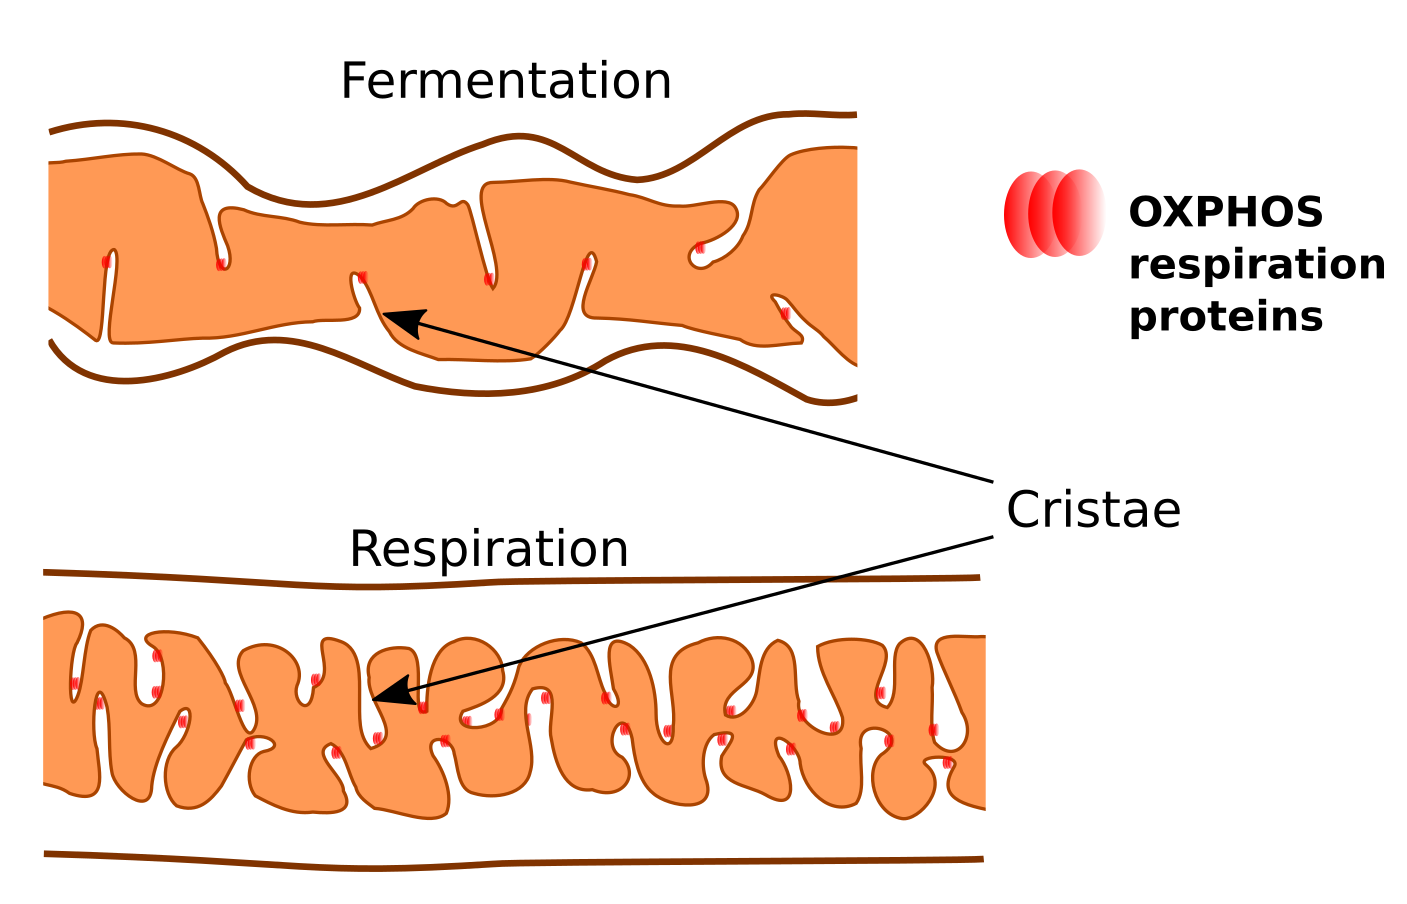
\includegraphics[width=.85\textwidth]{matrix}
    \caption[Mitochondria ultrastructure changes due to respiratory state]{Mitochondria in respiratory conditions display less heterogeneity in cristae density and tubule thickness compared to fermentative conditions.}\label{fig:matrix}
\end{figure}
%

It is interesting to note in our result that we see no significant differences in the heterogeneity characteristics of mitochondria tubules (both ΔΨ and tubule width) grown in the different respiratory conditions (i.e. glycerol+ethanol, lactate and raffinose). One possibility is that respiration states are similar in the three carbon sources, hence no changes in the IMM would be expected. Another possibility is that changes in the IMM are so subtle among the respiratory conditions that they are not resolvable by the optics of the system.

Between the two, we favor the second explanation because from our results in \Fref{ch:three}, we know that the respiration rates are different among the three respiratory carbon sources. One way to test this is to try to inhibit a respiration pathway that is specific to just a subset of the carbon sources. For example it is known that lactate oxidation happens directly at the \emph{lactate:cytochrome c} oxidoreductase complex. Yeast cells are able to grow normally on lactate substrate when given Antimycin A, a respiratory chain inhibitor that blocks the transfer of electrons to cytochrome b, which is positioned upstream of the \emph{lactate:cytochrome c} oxidoreductase complex. Thus it would be expected that under Antimycin A, yeast grown in raffinose would exhibit heterogeneity characteristics more similar to that of glucose (fermentation) while lactate would still retain normal respiratory heterogeneity characteristics. Yeast cells would not be able to grow in glycerol+ethanol when given Antimycin A as it has to undergo respiration.

Another interesting followup would be to use a fluorescent protein marker tagged to the ATP-synthase subunit (similar to the Jimenez study) and apply a membrane potential dye to see if the F1F0-cluster domains really co-localize with local membrane potential heterogeneity. One difficulty would be that we would not be able to use our mitochondrial matrix targeted marker with mRuby2 as the ATP-synthase would need to use the emission and excitation spectrum that mRuby2 lies in. This could be overcome by tagging either the ATP-synthase or the matrix targeted marker with a blue excitation/emission fluorescent protein.





